\documentclass{osa-article}
%!TEX root = ../thesis.tex
% !TEX TS-program = xelatex
% ****************************** Misc ******************************************
\usepackage{blindtext}
% ******************************************************************************
% ****************************** Custom Margin *********************************
% Add `custommargin' in the document class options to use this section
% Set {innerside margin / outerside margin / topmargin / bottom margin}  and
% other page dimensions

% Add spaces between paragraphs
%\setlength{\parskip}{0.5em}
% Ragged bottom avoids extra whitespaces between paragraphs
% To remove the excess top spacing for enumeration, list and description
%\usepackage{enumitem}
%\setlist[enumerate,itemize,description]{topsep=0em}

% *****************************************************************************
% ******************* Fonts (like different typewriter fonts etc.)*************
\usepackage{ wasysym }

% Add `customfont' in the document class option to use this section


% *****************************************************************************
% **************************** Custom Packages ********************************

% ************************* Algorithms and Pseudocode **************************

\usepackage{algpseudocode}


% ********************Captions and Hyperreferencing / URL **********************

% Captions: This makes captions of figures use a boldfaced small font.
%\RequirePackage[small,bf]{caption}

% \RequirePackage[labelsep=space,tableposition=top,small,bf]{caption}
% \renewcommand{\figurename}{Fig.} %to support older versions of captions.sty


% *************************** Graphics and figures *****************************

%\usepackage{rotating}
%\usepackage{wrapfig}

% Uncomment the following two lines to force Latex to place the figure.
% Use [H] when including graphics. Note 'H' instead of 'h'
%\usepackage{float}
%\restylefloat{figure}

% Subcaption package is also available in the sty folder you can use that by
% uncommenting the following line
% This is for people stuck with older versions of texlive
%\usepackage{sty/caption/subcaption}
\usepackage{subcaption}

% ********************************** Tables ************************************
\usepackage{booktabs} % For professional looking tables
\usepackage{multirow}

\usepackage{multicol}
\usepackage{longtable}
\usepackage{tabularx}


% *********************************** SI Units *********************************
\usepackage[allow-number-unit-breaks=true,separate-uncertainty=true,multi-part-units=single,binary-units=true]{siunitx} % use this package module for SI units

% ******************************* Line Spacing *********************************

% Choose linespacing as appropriate. Default is one-half line spacing as per the
% University guidelines

% \doublespacing
% \singlespacing

\usepackage{enumitem}

% ************************ Formatting / Footnote *******************************

% Don't break enumeration (etc.) across pages in an ugly manner (default 10000)
%\clubpenalty=500
%\widowpenalty=500

%\usepackage[perpage]{footmisc} %Range of footnote options


% *****************************************************************************
% *************************** Bibliography  and References ********************

%\usepackage{cleveref} %Referencing without need to explicitly state fig /table

% Add `custombib' in the document class option to use this section
% \ifuseCustomBib
   % \RequirePackage[numbers,sort&compress]{natbib} % CustomBib

% If you would like to use biblatex for your reference management, as opposed to the default `natbibpackage` pass the option `custombib` in the document class. Comment out the previous line to make sure you don't load the natbib package. Uncomment the following lines and specify the location of references.bib file


% \fi

% changes the default name `Bibliography` -> `References'


% ******************************************************************************
% ************************* User Defined Commands ******************************
% ******************************************************************************

% *********** To change the name of Table of Contents / LOF and LOT ************

%\renewcommand{\contentsname}{My Table of Contents}
%\renewcommand{\listfigurename}{My List of Figures}
%\renewcommand{\listtablename}{My List of Tables}


% ********************** TOC depth and numbering depth *************************




% ******************************* Nomenclature *********************************

% To change the name of the Nomenclature section, uncomment the following line

%\renewcommand{\nomname}{Symbols}


% ********************************* Appendix ***********************************

% The default value of both \appendixtocname and \appendixpagename is `Appendices'. These names can all be changed via:

%\renewcommand{\appendixtocname}{List of appendices}
%\renewcommand{\appendixname}{Appndx}

% *********************** Configure Draft Mode **********************************

% Uncomment to disable figures in `draft'
%\setkeys{Gin}{draft=true}  % set draft to false to enable figures in `draft'

% These options are active only during the draft mode
% Default text is "Draft"
%\SetDraftText{DRAFT}

% Default Watermark location is top. Location (top/bottom)
%\SetDraftWMPosition{bottom}

% Draft Version - default is v1.0
%\SetDraftVersion{v1.1}

% Draft Text grayscale value (should be between 0-black and 1-white)
% Default value is 0.75
%\SetDraftGrayScale{0.8}


% ******************************** Todo Notes **********************************
%% Uncomment the following lines to have todonotes.

% Example todo: \mynote{Hey! I have a note}

%%%
\usepackage{pgfplots}
\usepackage{tikzscale}
% \usepackage{helvet}

\pgfplotsset{
  tick label style = {font=\sansmath\sffamily\footnotesize},
  %every axis label = {font=\sansmath\sffamily},
  %legend style = {font=\sansmath\sffamily},
  %label style = {font=\sansmath\sffamily}
}
% https://github.com/matlab2tikz/matlab2tikz/issues/672
\newlength{\figwidth}
\newlength{\figheight}

\setlength{\figwidth}{0.4\textwidth}
\setlength{\figheight}{0.6180\figwidth}


\usepackage{graphicx}
\usepackage{xcolor}
\definecolor{darkblue}{rgb}{0,0,0.5}
\usepackage{transparent}

\usepackage{import}

\usepackage{pdflscape}

\usepackage{dpfloat}
\usepackage{multicol}

\usepackage{mhchem}
% \usepackage{wrapfig}
% \usepackage[super]{nth}


  % \newcommand{\nochapter}[1]{%
  %   \refstepcounter{chapter}%
  %   \addcontentsline{toc}{chapter}{\protect\numberline{\thechapter}#1}%
  %   \markright{#1}}


  \usepackage{tikz}
  \usepackage{graphicx}
  \usetikzlibrary{positioning}

%
% \usepackage[active,graphics]{preview}
%
% \usepackage{array}
% \makeatletter
% \font\dummyft@=dummy \relax
% \dummyft@
% \tracinglostchars=\z@
% \count@\sixt@@n
% \loop
% \ifnum\count@ >\z@
% \advance\count@\m@ne
% \textfont\count@\dummyft@
% \scriptfont\count@\dummyft@
% \scriptscriptfont\count@\dummyft@
% \repeat
% \let\selectfont\relax
% \let\mathversion\@gobble
% \let\getanddefine@fonts\@gobbletwo
% \pagestyle{empty}
% \let\ps@fancy\ps@empty
% \let\hline\relax
% \newcolumntype{|}{}
% \let\cleardoublepage\relax
% \makeatother

%!TEX root = ../thesis.tex

% \usepackage{makeidx}
\RequirePackage[xindy,acronym,toc,symbols]{glossaries-extra}

\makeglossaries{}
\makeindex

\setabbreviationstyle[acronym]{long-short}
\glssetcategoryattribute{acronym}{dualindex}{true}
\glssetcategoryattribute{general}{dualindex}{true}

% Symbols
\glsxtrnewsymbol[description={Field of View}]{FOV}{FOV}
\glsxtrnewsymbol[description={Rayleigh length}]{z_R}{\ensuremath{z_R}}
\glsxtrnewsymbol[description={Confocal parameter}]{b}{\ensuremath{b}}
\glsxtrnewsymbol[description={Half angle of the entrance pupil of a lens}]{alpha}{\ensuremath{\alpha}}
\glsxtrnewsymbol[description={Bessel function of the first kind}]{J_1}{\ensuremath{J_1}}
\glsxtrnewsymbol[description={Fluorescence molecule lifetime as a half life}]{tau}{\ensuremath{\tau}}
\glsxtrnewsymbol[description={Spot size of \gls{Gaussian beam}, waist}]{omega_0}{\ensuremath{\omega_0}}
\glsxtrnewsymbol[description={Wavelength}]{lambda}{\ensuremath{\lambda}}
\glsxtrnewsymbol[description={Numerical aperture}]{NA}{NA}
\glsxtrnewsymbol[description={Electric field}]{E}{\ensuremath{E}}
\glsxtrnewsymbol[description={Intensity,~\(\gls{E}^2\)}]{I}{\ensuremath{I}}
\glsxtrnewsymbol[description={Spot size of a Gaussian beam}]{w_0}{\ensuremath{w_0}}

%Computer vision
\glsxtrnewsymbol[description={World coordinates, \((X, Y, Z)\)}]{X}{\ensuremath{\mathbf{X}}}
\glsxtrnewsymbol[description={Camera-centered world coordinate,\((X_c, Y_c, Z_c)\), left camera}]{X_c}{\ensuremath{\mathbf{X_c}}}
\glsxtrnewsymbol[description={Camera-centered world coordinate,\((X_c', Y_c', Z_c')\) right camera}]{X_c'}{\ensuremath{\mathbf{X_c'}}}
\glsxtrnewsymbol[description={Ray to point on image plane,\((x,y,f)\), left camera}]{p}{\ensuremath{\mathbf{p}}}
\glsxtrnewsymbol[description={Ray to point on image plane,\((x,y,f)\), right camera}]{p'}{\ensuremath{\mathbf{p'}}}
\glsxtrnewsymbol[description={Image plane coordinates,\((x,y)\), left camera}]{x}{\ensuremath{\mathbf{x}}}
\glsxtrnewsymbol[description={Image plane coordinates,\((x,y)\), right camera}]{x'}{\ensuremath{\mathbf{x'}}}
\glsxtrnewsymbol[description={Pixel coordinates,\((u,v)\), left camera}]{w}{\ensuremath{\mathbf{w}}}
\glsxtrnewsymbol[description={Pixel coordinates,\((u,v)\), right camera}]{w'}{\ensuremath{\mathbf{w'}}}
\glsxtrnewsymbol[description={Camera parameters, left camera}]{K}{\ensuremath{\mathbf{K}}}
\glsxtrnewsymbol[description={Camera parameters, right camera}]{K'}{\ensuremath{\mathbf{K'}}}

\glsxtrnewsymbol[description={Rotation matrix (orthonormal)}]{R}{\ensuremath{\mathbf{R}}}
\glsxtrnewsymbol[description={Translation vector (3 element)}]{T}{\ensuremath{\mathbf{T}}}
\glsxtrnewsymbol[description={The Fundamental matrix}]{F}{\ensuremath{\mathbf{F}}}
\glsxtrnewsymbol[description={The Essential matrix}]{Essential}{\ensuremath{\mathbf{E}}}
\glsxtrnewsymbol[description={The Homography matrix}]{H}{\ensuremath{\mathbf{H}}}
\glsxtrnewsymbol[description={\(3\times3\) matrix containing coordinates from \gls{T}}]{T_x}{\ensuremath{\mathbf{T_\times}}}
\glsxtrnewsymbol[description={Mean square error: \(\operatorname{MSE}=\frac{1}{n}\sum_{i=1}^n{(Y_i-\hat{Y_i})}^2\)}]{MSE}{\ensuremath{MSE}}

\glsxtrnewsymbol[description={Tissue viscosity}]{eta_1_visc}{\ensuremath{\eta_1}}
\glsxtrnewsymbol[description={Cellular viscosity}]{eta_2_visc}{\ensuremath{\eta_2}}
\glsxtrnewsymbol[description={Time constant of the tissue}]{tau_visc}{\ensuremath{\tau}}
\glsxtrnewsymbol[description={Ensemble stiffness}]{E_visc}{\ensuremath{E}}

% Mean Square Error
% Glossary

\newglossaryentry{4f}{
    name={4f},
    description={Two lens system with each plane separated by a focal length \(f \)}
}
\newglossaryentry{primary imaging plane}{
    name={primary imaging plane},
    description={The first plane where a true image is relayed.}
}
\newglossaryentry{objective lens}{
    name={objective lens},
    description={The collecting lens nearest the sample}
}
\newglossaryentry{specificity}{
    name={specificity},
    description={The ability of fluorescent imaging to label specific aspects of a sample}
}
\newglossaryentry{depth of field}{
    name={depth of field},
    description={The axial range about a lens' focal plane where an image sample will continued to keep focus.}
}
\newglossaryentry{airy disk}{
    name={Airy disk},
    description={Theoretical lateral intensity distribution of a point emitter}
}
\newglossaryentry{nyquist sampling theory}{
    name={Nyquist sampling theory},
    description={The resolution of the detector required to resample the image information faithfully is twice the..}
}
\newglossaryentry{stokes shift}{
    name={stoke shift},
    description={The red shift in colour of fluorescent molecules when emission light is compared to excitation light.}
}
\newglossaryentry{autophagy}{
    name={autophagy},
    description={The mechanism by which cells disassemble.}
}
\newglossaryentry{lysosome}{
    name={lysosome},
    description={Organelle within the cell where enzymes are kept for degrading molecules}
}
\newglossaryentry{transfection}{
    name={transfection},
    description={The process by which external matter is inserted into the cell}
}
\newglossaryentry{etendue}{
    name={etendue},
    description={A property of propagating light which is conversed and is defined as the product solid angle of of the system's entrance pupil and the area}
}
\newglossaryentry{coherent}{
    name={coherent},
    description={The distance over which a photons from the same source will stay in phase}
}
\newglossaryentry{super-continuum laser}{
    name={super-continuum laser},
    description={A source of white laser light, achieved using non-linear effects in a photonic crystal fibre and a pump laser.}
}
\newglossaryentry{pixel}{
    name={pixel},
    description={Picture element}
}
\newglossaryentry{photosite}{
    name={photosite},
    description={Single light recording element of an array forming an imaging detector}
}

\newglossaryentry{wide-field}{
    name={wide-field},
    description={The entire area of interest is exposed to light and recorded at once}
}
\newglossaryentry{quantum efficiency}{
    name={quantum efficiency},
    description={The photonic to electron conversion rates, the \emph{yield} of the detector}
}
\newglossaryentry{dynamic range}{
    name={dynamic range},
    description={The ratio between the largest and smallest intensity values that a photo-site can assume}
}
\newglossaryentry{bit depth}{
    name={bit depth},
    description={The resolution in bits of a digitally converted measurand}
}
\newglossaryentry{dark current}{
    name={dark current},
    description={The residual electric current flowing in each photo-site when there is no incident illumination}
}
\newglossaryentry{read noise}{
    name={read noise},
    description={Noise contribution from the electronics within the camera}
}
\newglossaryentry{photon noise}{
    name={photon noise},
    description={The intrinsic variation of the incident photon flux}
}
\newglossaryentry{poissonian distribution}{
    name={poissonian distribution},
    description={Discrete probability distribution in a fixed epoch}
}
\newglossaryentry{fluorophore}{
    name={fluorophore},
    description={Fluorescent molecule: chromophore, fluorochrome}
}
\newglossaryentry{photosensitier}{
    name={photosensitier},
    description={Molecules which produce chemical change is surrounding molecules using photon energy}
}
\newglossaryentry{confocal microscope}{
    name={confocal microscope},
    description={A laser scanning microscope wherein an adjustable pinhole is placed at a conjugate imaging plane to control axial and spatial resolution of the reconstructed image}
}
\newglossaryentry{confocal}{
    name={confocal},
    description={Common focal point between lenses, similiar to conjugate planes}
}
\newglossaryentry{galvanometric scanning mirrors}{
    name={galvanometric scanning mirrors},
    description={Voltage controlled mirrors where voltage is proportional to angle}
}
\newglossaryentry{resonant scanning mirrors}{
    name={resonant scanning mirrors},
    description={Voltage controlled mirrors driven at their resonant frequency to increase the maximum viable scanning speed}
}
\newglossaryentry{photobleaching}{
    name={photobleaching},
    description={The ensemble reduction in fluorescent intensity as individual \gls{fluorophore}s lose the ability to fluoresce}
}
\newglossaryentry{photo-toxicity}{
    name={photo-toxicity},
    description={Damage caused to a biological sample due to light}
}
\newglossaryentry{aberration}{
    name={aberration},
    description={Distortions caused in an image by imperfect optics in the imaging system}
}
\newglossaryentry{Fourier transform}{
    name={Fourier transform},
    description={Coordinate transform to convert points in real space into points in frequency space}
}
\newglossaryentry{missing cone}{
    name={missing cone},
    description={The cone of space missing in the 3D \gls{OTF}}
}
\newglossaryentry{super-resolution}{
    name={super-resolution},
    description={Imaging at resolutions beyond the diffraction limit}
}
\newglossaryentry{light-sheet}{
    name={light-sheet},
    description={A thin plane of light}
}
\newglossaryentry{convolution theorem}{
    name={convolution theorem},
    description={The relation between convolution in Cartesian space versus multiplication in frequency space, see Appendix~\ref{appendix:convolution_theorem}}
}
\newglossaryentry{epi-fluorescence}{
    name={epi-fluorescence},
    description={Fluorescence microscopy imaged along the same optics used to illuminate}
}
\newglossaryentry{optical sectioning}{
    name={optical sectioning},
    description={The ability of a microscope to image axial slices of a thick sample}
}
\newglossaryentry{ultra-microscope}{
    name={ultra-microscope},
    description={A light-sheet microscope for observing small particles or colloids using scattered light, developed by R. A. Zsigmondy 1902}
}
\newglossaryentry{openSPIM}{
    name={openSPIM},
    description={Open hardware project of documentation to help home-users build their own \gls{SPIM}}
}
\newglossaryentry{Gaussian beam}{
    name={Gaussian beam},
    description={Model that governs the propagation of \emph{vanilla} coherent \gls{Laser} sources with no phase of illumination shaping optics.}
}
\newglossaryentry{Lorentzian}{
    name={Lorentzian},
    description={\(f(x) = \frac{1}{x^2+1}\)
    }
}
\newglossaryentry{Rayleigh length}{
    name={Rayleigh length},
    description={The distance along the propagation direction of a Gaussian beam where the beam is percieved to be still collimated.
    }
}
\newglossaryentry{virtual light-sheet}{
    name={virtual light-sheet},
    description={\Gls{light-sheet} generated by spatially sweeping a beam}
}
% \newglossaryentry{tele-centric}{
%     name={tele-centric},
%     description={A lens property where all the chief rays are collimated and parallel to the optical axis}
% }
\newglossaryentry{working distance}{
    name={working distance},
    description={The distance an objective needs to be away from a sample to keep focus, distance to the focal plane}
}
\newglossaryentry{tomography}{
    name={tomography},
    description={Tomography is imaging of a sample by sections or sectioning using waves}
}
\newglossaryentry{Spatial Light Modulator}{
    name={Spatial Light Modulator},
    description={Array device for modulating phase and/or intensity of incident light}
}
\newglossaryentry{exotic beam}{
    name={exotic beam},
    description={Non-Gaussian beams with structure and exploitable properties}
}
\newglossaryentry{axicon}{
    name={axicon},
    description={Lens with a conical surface}
}
\newglossaryentry{Bessel beam}{
    name={Bessel beam},
    description={Non-diffraction, self-healing beam. Narrow central lobe with multiple outer orders}
}
\newglossaryentry{Airy beam}{
    name={Airy beam},
    description={Non-diffraction, self-healing beam. Appears to bend}
}
\newglossaryentry{comatic aberration}{
    name={comatic aberration},
    description={Abberation caused from imaging off-axis}
}
\newglossaryentry{lattice light-sheet}{
    name={lattice light-sheet},
    description={Lattice of self-reinforced Bessel beams, narrowed into a sheet}
}
\newglossaryentry{deconvolution}{
    name={deconvolution},
    description={The mathematical reversing of convolution. Improves image fidelity}
}
\newglossaryentry{Laser}{
    name={laser},
    description={Light Amplification by Stimulated Emission}
}
\newglossaryentry{LabVIEW}{
    name={LabVIEW},
    description={Graphical programming language for lab rapid development instrumentation}
}
\newglossaryentry{imaging board}{
    name={imaging board},
    description={Top most breadboard, holding imaging and illumination optics}
}
\newglossaryentry{illumination board}{
    name={illumination board},
    description={Bottom most breadboard, holding illumination sources and optics}
}
\newglossaryentry{imaging optical rail}{
    name={imaging optical rail},
    description={Optical rail holing camera and filter wheel}
}
\newglossaryentry{detection arm}{
    name={detection arm},
    description={\SI{45}{\degree} opts-mechanics rail on the imaging board holding detection optics}
}
\newglossaryentry{illumination arm}{
    name={illumination arm},
    description={\SI{45}{\degree} opts-mechanics rail on the imaging board holding illumination optics}
}
\newglossaryentry{telecentric}{
    name={telecentric},
    description={A lens property where all the chief rays are collimated and parallel to the optical axis}
}
\newglossaryentry{state machine}{
    name={state machine},
    description={A model of computation containing a finite number of possible states of which it may only exist in one at any time.}
}
\newglossaryentry{producer-consumer architecture}{
    name={producer-consumer architecture},
    description={Parallel running \gls{state machine}s, where the producer machine sends commands and data to the consumer machine}
}
\newglossaryentry{queueing architecture}{
    name={queueing architecture},
    description={Operations and data are queued into a register for action upon from a state machine. Queues may be first in first out, first in last out etc.}
}
\newglossaryentry{race conditions}{
    name={race conditions},
    description={When system attempts to perform two or more operations at the same time}
}
\newglossaryentry{enumerated type}{
    name={enumerated type},
    description={A variable which acts as an identifer and acts as a constant value}
}
\newglossaryentry{exposure time}{
    name={exposure time},
    description={Integration time of a single recorded frame}
}
\newglossaryentry{exposure}{
    name={exposure},
    description={Exposure time \(\times \) gain}
}
\newglossaryentry{background signal}{
    name={background signal},
    description={Additional signal from the environment, specimen or system which contributes to lowering the \gls{SNR}}
}
\newglossaryentry{homography}{
    name={homography},
    description={A projective transform}
}
\newglossaryentry{Ram-Lak filter}{
    name={Ram-Lak filter},
    description={Linear real (amplitude) ramp filter in Fourier space}
}
\newglossaryentry{sinugram}{
    name={sinogram},
    description={The image of Cartesian as transformed into angular space}
}
% \newglossaryentry{homography matrix}{
%     name={homography matrix},
%     description={DEFINE}
% }
\newglossaryentry{homogeneous coordinates}{
    name={homogeneous coordinates},
    description={A higher dimensional representation of lower dimensional coordinates to facilitate non-linear operations}
}
\newglossaryentry{zebrafish}{
    name={zebrafish},
    description={\emph{Danio rerio}. A model organism  ubiquitous in light-sheet imaging}
}
\newglossaryentry{chorion}{
    name={chorion},
    description={The soft membrane surrounding embryos}
}
\newglossaryentry{sample plane}{
    name={sample plane},
    description={Plane in sample as imaged onto the imaging plane of an optical system}
}
\newglossaryentry{world point}{
    name={world point},
    description={A point in world-centered coordinates}
}
\newglossaryentry{essential matrix}{
    name={essential matrix},
    description={\(3\times 3\) matrix which relates corresponding points in stereo image pairs in calibrated cameras}
}
\newglossaryentry{fundamental matrix}{
    name={fundamental matrix},
    description={\(3\times 3\) matrix which relates corresponding points in stereo image pairs}
}
\newglossaryentry{image plane}{
    name={image plane},
    description={Image one focal distance away from the camera-centered coordinates along the optical axis}
}
\newglossaryentry{Radon transform}{
    name={Radon transform},
    description={Integral transform converting Cartesian space into angular space along one axis}
}
\newglossaryentry{agarose VII}{
    name={agarose VII},
    description={Optical clear hydrated gel. This type of agarose is the closest matching refractive index to that of water}
}
\newglossaryentry{slit-scanning}{
    name={slit-scanning},
    description={The scanning of a narrow slit to increase contrast and resolution along the direction orthogonal to the slit direction}
}
\newglossaryentry{3D printing}{
    name={3D printing},
    description={Additive method of building shapes, often using hot malleable plastic extrusions}
}
% \newglossaryentry{ABS}{
%     name={ABS},
%     description={DEFINE}
% }
% \newglossaryentry{PLA}{
%     name={PLA},
%     description={DEFINE}
% }
\newglossaryentry{organoid}{
    name={organoid},
    description={A miniature and simplified organ}
}
\newglossaryentry{SH-SY5Y}{
    name={SH-SY5Y},
    description={Human derived neuronal cell line}
}
\newglossaryentry{open-hardware}{
    name={open-hardware},
    description={Freely and open available designs for hardware}
}
\newglossaryentry{virion}{
    name={virion},
    description={A single virus particle}
}
\newglossaryentry{capsid}{
    name={capsid},
    description={Protein shell of a virus}
}
\newglossaryentry{VP26}{
    name={VP26},
    description={Structural protein found in the capsid}
}
\newglossaryentry{VP1/2}{
    name={VP1/2},
    description={Structural protein found in the capsid}
}
\newglossaryentry{VP16}{
    name={VP16},
    description={Tegument protein which complexes with host DNA to induce gene transcription, the initiation of gene expression}
}
%\gls{background fluorescence}
% Acronyms

% \newacronym{FOV}{FOV}{Field of View}
\newacronym{sCMOS}{sCMOS}{scientific Complementary Metal-Oxide-Semiconductor}
% \newacronym{NA}{NA}{Numerical Aperture}
\newacronym{SNR}{SNR}{Signal to Noise ratio}
\newacronym{CCD}{CCD}{Charge-coupled device}
\newacronym{ICCD}{ICCD}{Intensified Charge-coupled device}
% \newacronym{Laser}{Laser}{Light Amplification by Stimulated Emission}
\newacronym{LED}{LED}{Light Emitting Diode}
\newacronym{EMCCD}{EMCCD}{Electron-Multiplying Charge-Coupled Device}
\newacronym{CMOS}{CMOS}{Complementary Metal-Oxide-Semiconductor}
\newacronym{FRAP}{FRAP}{Fluorescence Recovery After Photobleaching}
\newacronym{2P}{2P}{2-Photon}
\newacronym{SIM}{SIM}{Structured Illumination Microscopy}
\newacronym{iSIM}{iSIM}{instant Structured Illumination Microscopy}
\newacronym{mSIM}{mSIM}{multi-focal Structured Illumination Microscopy}
\newacronym{OTF}{OTF}{Optical Transfer Function}
\newacronym{LSFM}{LSFM}{\Gls{light-sheet} Fluorescence Microscopy}
\newacronym{SPIM}{SPIM}{Selective Plane Imaging Microscope}
\newacronym{FWHM}{FWHM}{Full-Width at Half-Maximum}
\newacronym{DSLM}{DSLM}{Digitally scanned Light-Sheet Microscopy}
\newacronym{ETL}{ETL}{Electronically Tuneable Lens}
\newacronym{iSPIM}{iSPIM}{inverted Selective-Plane Imaging Microscope}
\newacronym{LWD}{LWD}{Long Working Distance}
\newacronym{diSPIM}{diSPIM}{dual inverted Selective-Plane Imaging Microscope}
\newacronym{MuVi-SPIM}{MuVi-SPIM}{Multiview Selective-Plane Illumination Microscope}
\newacronym{OPM}{OPM}{Oblique Plane Microscopy}
\newacronym{SLM}{SLM}{\gls{Spatial Light Modulator}}
\newacronym{PSF}{PSF}{Point Spread Function}
\newacronym{STED}{STED}{Simulated Emission Depletion}
\newacronym{mSPIM}{mSPIM}{multidirectional Selective Plane Illumination Microscopy}
\newacronym{SCAPE}{SCAPE}{Swept Confocally-Aligned Planar Excitation}
\newacronym{3D}{3D}{Three Dimensional}
\newacronym{2D}{2D}{Two Dimensional}
\newacronym{AOTF}{AOTF}{Acousto-Optic Tunable Filter}
% \newacronym{LabVIEW}{LabVIEW}{Laboratory Virtual Instrument Engineering Workbench}
\newacronym{TTL}{TTL}{Transistor-Transistor Logic}
\newacronym{DAQ}{DAQ}{Data Acquisition}
\newacronym{RS232}{RS232}{Recommended Standard 232}
\newacronym{FEP}{FEP}{Fluorinated Ethylene Propylene}
\newacronym{CAD}{CAD}{Computer Aided Design}
\newacronym{OPT}{OPT}{Optical Projection Tomography}
\newacronym{eOPT}{eOPT}{emission Optical Projection Tomography}
\newacronym{tOPT}{tOPT}{transmission Optical Projection Tomography}
\newacronym{SVD}{SVD}{Singular Value Decomposition}
\newacronym{SPT}{SPT}{Single Particle Tracking}
\newacronym{FFT}{FFT}{Fast Fourier Transform}
\newacronym{PBS}{PBS}{Phosphate-Buffered Saline}
\newacronym{HSV}{HSV}{Herpes Simplex Virus}
\newacronym{INM}{INM}{Inner Nuclear Membranes}
\newacronym{ONM}{ONM}{Outer Nuclear Membranes}
\newacronym{TIRF}{TIRF}{Total Internal Reflection Fluorescence}
\newacronym{PFV}{PFV}{Prototype Foamy Virus}
\newacronym{HILO}{HILO}{Highly Inclined and Laminated Optical sheet}
\newacronym{dSTORM}{dSTORM}{\emph{direct} stochastic optical reconstruction microscopy}
\newacronym{NN}{NN}{Neural Network}
\newacronym{EM}{EM}{Electron Microscopy}
\newacronym{AFM}{AFM}{Atomic Force Microscopy}
\newacronym{FLIM}{FLIM}{Fluorescence Lifetime Imaging Microscopy}
\newacronym{ABS}{ABS}{Acrylonitrile Butadiene Styrene}
\newacronym{PLA}{PLA}{Polylactic acid}
\newacronym{RAM}{RAM}{Random Access Memory}

\newacronym{Rac1}{Rac1}{Ras-related C3 botulinum toxin substrate 1}
\newacronym{DNRAC}{DNRAC}{dominant-negative Rac1gene construct}
\newacronym{DNROCK}{DNROCK}{dominant-negative Rho-kinase construct}
\newacronym{MoECad}{MoECad}{Ras-related C3 botulinum toxin substrate 1}
\newacronym{RhoA}{RhoA}{Ras homolog gene family, member A}
\newacronym{WT}{WT}{wild type}
\newacronym{GFP}{GFP}{Green Fluorescent Protein}
\newacronym{PFA}{PFA}{paraformaldehyde}
\newacronym{flOPT}{flOPT}{frame localisation Optical Projection Tomography}
% \newacronym{MoECad}{MoECad}{}
% \newacronym{LWD}{LWD}{Long Working Distance}


\makeatletter
\renewcommand*\env@matrix[1][*\c@MaxMatrixCols c]{%
   \hskip -\arraycolsep
   \let\@ifnextchar\new@ifnextchar
   \array{#1}}
\makeatother

%% Select the journal you're submitting to
%% oe, boe, ome, osac, osajournal
\journal{osajournal}
% Key:
% Express journals must have the correct journal selected:
% {oe} Optics Express
% {boe} Biomedical Optics Express
% {ome} Optical Material Express
% {osac} OSAC Continuum
% Other OSA journals may use:
% {osajournal} Applied Optics, Advances in Optics and Photonics, Journal of the Optical Society of America A/B, Optics Letters, Optica, Photonics Research

% Uncomment if submitting to Photonics Research.
% ONLY APPLICABLE FOR \journal{osajournal}
% \setprjcopyright

% Set the article type
\articletype{Research Article}
% Note that article type is not required for Express journals (OE, BOE, OME and OSAC)

\begin{document}

\title{Frame Localisation Optical Projection Tomography}

\author{Craig Russell,\authormark{1*,2}, \author{Pedro P Vallejo\authormark{1}}, Eric Rees,\authormark{1}}

\address{Department of Chemical Engineering and Biotechnology, University of Cambridge,\authormark{1}}
\address{National Physical Laboratory, \authormark{2}}
\email{\authormark{*}craig.russell@npl.co.uk} %% email address is required

% \homepage{http:...} %% author's URL, if desired

%%%%%%%%%%%%%%%%%%% abstract %%%%%%%%%%%%%%%%
\begin{abstract}
  We present a tomographic reconstruction algorithm, which is applied to Optical Projection Tomography (OPT) [1] images, that is robust to mechanical jitter and systematic angular and spatial drift.
  OPT relies on precise mechanical rotation and is less mechanically stable than large scale CT scanning systems, leading to reconstruction artefacts.
  The algorithm uses multiple (5+) tracked fiducial beads to recover the sample pose and the image rays are then back-projected at each orientation.
  The quality of the image reconstruction using the proposed algorithm shows an improvement when compared to the Radon transform.
  When adding a systematic spatial and angular mechanical drift, the reconstruction using the proposed algorithm shows a significant improvement over the Radon transform.
\end{abstract}


%%%%%%%%%%%%%%%%%%%%%%%%%%  body  %%%%%%%%%%%%%%%%%%%%%%%%%%

% \section{Frame localisation optical projection tomography}

% % \epigraph{\emph{Pascale Sauvage}}{--- Pablo Vallejo}
%
% % Volumetric imaging can also be achieved by rotating a sample and %reconstructing tomographically.
% % tomographically reconstructing the 3D distribution of a signal (scattering, absorption or luminosity) within the specimen.
% %Orthogonal imaging schema can be replaced with pass through imaging provide samples are sufficiently transparent.
% %Instead of scanning these samples laterally one can rotate their sample and reconstruct a full three dimensional image.
% %As tomographic technology has been shrunk to the millimeter scale, errors induced by hardware become apparent.
% Accurate %reconstructions of volumes rely on
% tomographic reconstruction relies
% heavily on precision movement and rotation.
% %This chapter addresses a key downside in traditional approaches to performing full three dimensional reconstructions tomographically.
% Here an algorithm will be presented that relies exclusively on multiple (4+) tracked fiducial beads to enable accurate reconstruction even with systematic mechanical drift.
% It will be demonstrated on ground truth simulated testcard image data with motion errors compounded onto the tomographic rotation.
% These motion errors will include systematic mechanical drift, giving a spiral path; and angular drift giving precession.

% \section{Rotational computer tomography in microscopy}

%Well establishjed
%Three-dimensional imaging of anatomy in thick biological samples provides valuable data for developmental biology studies.
%Tomographic techniques that generate 3D reconstructions from 2D images such as computed tomography (CT) and magnetic resonance imaging (MRI) are essential in medical applications to visualize morphology in large tissues and organs.
%CT and especially micro-CT can achieve micron-scale resolution using certain contrast agents, however the high doses of radiation used make this unsuitable for repeated experiments on a biological sample.
%Micro-MRI can also achieve resolution in the micron scale, however the cost and size of MRI instruments can be prohibitive for many applications[21].
%Furthermore, neither of these techniques can exploit the plethora of information that can be extracted through fluorescence microscopy.

Sharpe~\emph{et.al} proposed \gls{OPT}~\cite{sharpeOpticalProjectionTomography2002}
using visible light to image transparent or translucent mesoscopic samples, with micrometer resolution.
\gls{OPT} addresses the scale gap between photographic techniques (for samples typically larger than \SI{10}{\milli\meter}), and light microscopy techniques (samples smaller than \SI{1}{\milli\meter}) to image biological samples in the \SIrange{1}{10}{\milli\meter} regime.
% \gls{OPT} is non-invasive optically but may require specialist invasive preparation for its samples.

%Optical Projection Tomography was first proposed by Sharpe in 2002 [30]; it uses visible light to image and create volumetric data of transparent (naturally or artificially) mesoscopic objects (1 - 10 mm) at micron-level resolution.

\gls{OPT} is based on computerised tomography techniques~\cite{kakPrinciplesComputerizedTomographic2001} in which a set of projections of a specimen are imaged as the specimen travels through a full rotation.
Typically a Radon transform used to then transform this set of images into a 3D image stack in Cartesian (\(X,Y,Z\)).
%A cross-sectional stack of slices from the original object is reconstructed using a back-projection algorithm from the projection images.
The \gls{Radon transform} relies heavily on the assumption of circular motion with constant angular steps about a vertical axis.
This work presents an improved reconstruction algorithm that is robust to spatial and angular mechanical drifts during acquisitions, as well as inconsistent angular steps.

The proposed algorithm works by triangulating points between images pairs to extract camera pose using the theoretical framework used in stereoscopic imaging.

% There are two imaging modalities for \gls{OPT}, \gls{eOPT} and \gls{tOPT}.
% In \gls{eOPT}, a fluorescent sample is excited using an illumination source off axis to the detection, similar to \gls{light-sheet} but the entire \gls{depth of field} of the detection of objective is illuminated.
% % without the excitation being shaped into a sheet.
% Scattered illumination photons are rejected at the detector using an appropriate filter.
% In tOPT, a white-light source with a diffuser and a collimator is placed along the optical axis to provide near-collimated, uniform illumination onto the sample for transmission to a detector opposite (see \figurename~\ref{fig:OPT_digram}).
% Each \gls{photosite} at the detector corresponds to a ray that has passed through the sample and been attenuated by the sample.
% The \gls{eOPT} and \gls{tOPT} modes can work in unison to provide contextual information, with the transmission images indicating overall structure (optical density of absorption or scattering) which can be supplemented by the fluorescent signal from a label of interest.
%
% \begin{figure}
%   \centering
%   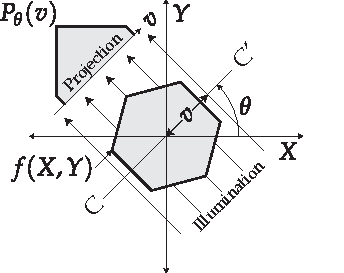
\includegraphics{./figures/OPT_digram}
%   \caption[Principle of OPT]{Principle of \gls{OPT}, a respective rotation between the sample and the detector illumination pair is iterated.
%   The volumetric image is later reconstructed from the set of detections (1/2D).}
%   \label{fig:OPT_digram}
% \end{figure}


\section{Stereoscopic imaging}

\begin{figure}
    \centering
    \begin{subfigure}[t]{0.48\textwidth}
        \centering
        \includegraphics{./figures/coordinate_system}
        \caption[Coordinate system]{Coordinate system used in this chapter describing a camera with an associated image plane one focal distance \(f\) away, imaging an object at point \(\gls{X}\).
        }\label{fig:coordinate_system_flopt}
    \end{subfigure}\hfill
    \begin{subfigure}[t]{0.48\textwidth}
      \centering
      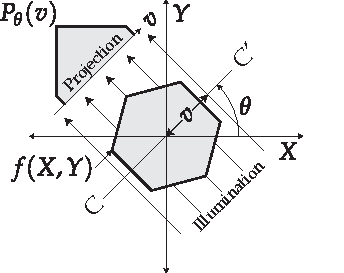
\includegraphics{./figures/OPT_digram}
      \caption[Principle of OPT]{From an angle \(\theta \), an object \(f(X,Y)\) and its projection \(P_\theta(t)\) are known.}\label{fig:OPT_digram}
      %{Principle of \gls{OPT}, a respective rotation between the sample and the detector illumination pair is iterated.
      % The volumetric image is later reconstructed from the set of detections (1/2D).}
    \end{subfigure}
    \caption[Coordinates and \gls{OPT}]{\gls{X_c} = \((X_c,Y_c,Z_c)\) is the camera-centered coordinate point in 3D space.
            \gls{X} = \((X,Y,Z)\) is the world coordinate point in 3D space.
            \gls{p} = \((x,y,f)\) is the ray vector to point of image plane.
            \gls{x} = \((x,y)\) is the image plane coordinates.
            \gls{w} = \((u,v)\) is the pixel coordinates (not shown) corresponding to the point \gls{x}.
            The optical axis travels along the \(Z_c\) axis through the image plane.}
    % \label{fig:aa}
\end{figure}
\begin{figure}
  \centering
  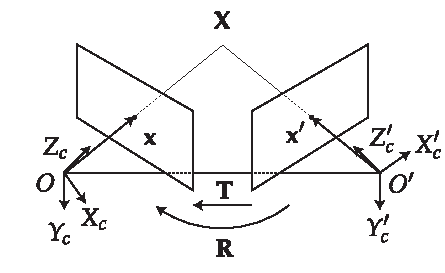
\includegraphics{./figures/epi-polar-geom}
  \caption[Epi-polar geometry described for two adjacent views]{
  Epi-polar geometry described for two adjacent views (or cameras of a scene).
  Coordinates as expressed in \figurename~\ref{fig:coordinate_system_flopt} with prime notation (\('\)) denoting the additional right camera view.
  Transforming from right to left camera-centered coordinates (\gls{X_c'} to \gls{X_c}) requires a rotation (\gls{R}) and a translation (\gls{T}).
  }\label{fig:epi-polar-geom}
\end{figure}

%\subsection{Projective geometry}

%Camera imaging is governed by projective geometry
%Parallel lines project onto a camera will have a vanishing point at the horizon.

%\subsection{Camera projections}

%\todo{Camera projections \ lecture notes 3}

The stereoscopic imaging scenes allows for the triangulation of individual features in three dimensional space (know as world points) when the features or fiducial markers in one detector are uniquely identifiable, see Figure~\ref{fig:epi-polar-geom} for the coordinate system which descibes this geometry. %(such as fluorescent beads).
Triangulation requires that each feature is detected in both images of a stereo imaging system, and for these detections to be correctly associated with one another, this is known as the correspondence problem.
Many methods exist to ensure that features are detected from image data and accurately associated between two cameras or views.
Properties of scale independent features and their surrounding pixel environment in one image can be matched to a similar feature in the second image.

%TODO ADD SOME STEREOIMAGING STUFF?



%TODO INSERT H E F DEFINTIONS
Coordinates in two adjaceent views with a common epi-pole (see Figure~\ref{fig:epi-polar-geom}) are related by the Essential matrix (\gls{Essential}) for uncalibrated cameras and the Fundamental matrix (\gls{F}) for calibrated cameras.
Their properties can described by:
\begin{gather}
\gls{p'}^T \gls{Essential} \gls{p} = 0 \label{eq:pEp}\\
\gls{Essential} = \gls{K'}^T \gls{F} \gls{K} %= \gls{T_x} \gls{R} = \mathbf{U}\Lambda \mathbf{V}^T%\gls{R} = U\LambdaV^T\\
\end{gather}
Where \(\gls{K}\) is a matrix which converts image plane coordinates to camera pixel coordinates and where \gls{p} refers to a point in the image plane.

\section{The proposed algorithm}

%The rotation may also not be orthogonal to the plane of detection.
The shift of a camera around a scene separated by a transformation matrix (\( \begin{bmatrix}[c|c] \gls{R} & \gls{T} \end{bmatrix}\)) is analogous to transforming the sample in the fixed view of an imaging detector, as in an \gls{OPT} acquisition. %TODO Reword
During an ideal \gls{OPT} acquisition, a marker will appear to follow an elliptical path in the \(xy\) image plane.
During the following volume reconstruction there is a fitting step to recover the path of the fiducial marker, which is used to apply as a correction before using the inverse \gls{Radon transform}.
This type of reconstruction not only ignores any mechanical jitter of the sample but also any affine, systematic, mechanical drift (in \(X,Y,Z,\theta,\phi,\psi \)). %TODO is this true?

Using two adjacent images of a scene, separated by some rotation and translation, world points in 3D space may be triangulated within the scene given the rotational and translational matrices of the respective camera views.

% The inverse is also possible, given a sufficient number of known fiducial points in a scene the translation and rotation matrices can be recovered.

% The recovery of a more exact description of the motion of the scene can eliminate any need for a fitting and may recover and correct for drift, as well as eliminate any mechanical jitter.
% Errors may however then be introduced from fiducial markers mechanically slipping and localisation errors.
% Fiducial markers in this sense refer to an accurately locatable marker common through different views in a sample.

Once a sufficient amount of fiducial markers are reliably tracked from the first to the second image, either of the \glslink{fundamental matrix}{fundamental} or \glslink{essential matrix}{essential} matrices can be computed.
Using the factorisation one of these matrixes, between each adjacent view of a rotating scene, the translation and rotational matrices can be recovered.
% Here we will discuss a reconstruction using \gls{F} but the same principle applies for \gls{Essential} and \gls{H}.

% Here are two ways of reconstructing using the fundamental matrix as described above.
To reconstruct we compute \gls{F} for the current image and the first image using 5 or more fiducial markers; having additional beads helps to remove ambiguity and increase confidence in \gls{F}.
Once \gls{F} is calculated \gls{F} is then decomposed into \(\gls{R}_n\) and \(\gls{T}_n\) between each view \(n\) and \(n+1\).
The image at view \(n+1\) is then back projected along the virtual optical axis within a virtual volume where the sample will be reconstructed.
The size of this back projection and virtual volume is chosen to be suitably large (so that important data is not lost).
% Then, all the prior rotation and translation matrices are serially multiplied from \(\begin{bmatrix}[c|c] \gls{R}_0&\gls{T}_0 \end{bmatrix}\) until \(\begin{bmatrix}[c|c] \gls{R}_n&\gls{T}_n \end{bmatrix}\) % \([R_n|T_n] \)
% , this final matrix is inverted and applied to the back projected volume.
The transformation matrices that are recovered are then inverted to realign the back projection of the image rays in the volume to their respective source positions.
% This process is repeated for every angle the sum of these ray projection volumes is filtered using a high-pass filter; here a \gls{Ram-Lak filter} is used.
% \footnote{Linear real (amplitude) ramp filter in Fourier space}. %: \(|v|\)}
% By producing a series of transformation matrices from adjacent acquisitions, errors compound and the reconstruction of volumes degrades with more projections, see \figurename~\ref{fig:irandons}.

\begin{figure}
    \centering
    \begin{subfigure}[t]{\textwidth}
      \centering
      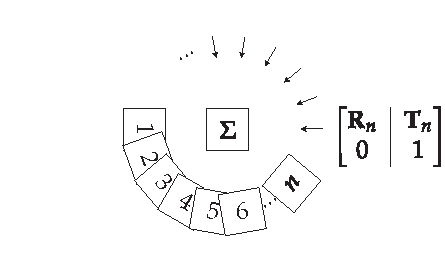
\includegraphics{./figures/flopt_algorithm_forward}
      \caption{Forward model}\label{fig:flopt_algorithm_forward}
    \end{subfigure}\\\vspace{\abovecaptionskip}
    \begin{subfigure}[t]{\textwidth}
      \centering
      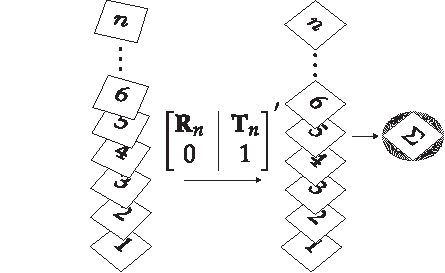
\includegraphics{./figures/flopt_algorithm}
      \caption{Reconstruction method, solving the inverse problem.}\label{fig:flopt_algorithm_inverse}
    \end{subfigure}
    \caption[Simulation of \gls{OPT} data incorporating rotational and translational offsets, and the proposed reconstruction algorithm]{
    % Two dimensional representation of the reconstruction algorithm.
    This figure illustrates the simulation of \gls{OPT} data incorporating rotational and translational offsets, and the proposed reconstruction algorithm.
    (\subref{fig:flopt_algorithm_forward}): The \(n\) projections of the object (\(\Sigma \)), at rotation (\(\gls{R}_1\) to \(\gls{R}_n\)) and translation (\(\gls{T}_1\) to \(\gls{T}_n\)), produces \(n\) frames of image data.
    During the \gls{OPT} measurement, \(n\) projections of the object \(\Sigma \) are observed with rotations \(\gls{R}_1\) to \(\gls{R}_n\) and corresponding translations \(\gls{T}_1\) to \(\gls{T}_n\) where the translations account for imperfect alignment.
    (\subref{fig:flopt_algorithm_inverse}): In the reconstruction algorithm, the rotational and translational matrices are recovered (\(\gls{R}_1'\) to \(\gls{R}_n'\) and \(\gls{T}_1'\) to \(\gls{T}_n'\)) from triangulation of the fiducial markers.
    These transformation matrices are then used to obtain a contribution to the volumetric reconstruction from each observed frame and the summated reconstruction is assembled from the \(n\) frames.
    The now realigned back projections are summed to produce an unfiltered back projection.
    % and inversely applied
    % to align back project the datasets,
    The transformation matrices are shown in augmented form using homogenous coordinates.
    }\label{fig:flopt_algorithm} %TODO tidy
\end{figure}

% The second approach is robust against compound errors but an additional programatic step is needed to know which beads in the first image correspond to beads in the \(n^{\text{th}}\) image.
% This can be is achieved using tracking and momentum particle tracking algorithms, though confounding issues can arise i.e.~if a particle orbits too far away from the imaging plane or occlusions occur.

In both cases a decomposed \gls{F} matrix will produce four possible transformation pairs (\gls{R},\gls{T}; \gls{R},-\gls{T}; -\gls{R},\gls{T}; -\gls{R},-\gls{T}). %TODO look this up.
Once the transformation matrix between the current view (\(n\)) and the first view is calculated the proceeding transformation matrices are then easily chosen by similarity to the previous collected matrix and general direction of motion.
An example of this type of selection would be:
\begin{align}
\min_{I(n)}\left[I(n) = \left(\begin{bmatrix}[c|c] \gls{R}_n&\gls{T}_n \end{bmatrix} - \begin{bmatrix}[c|c] \gls{R}_{n-1}&\gls{T}_{n-1} \end{bmatrix}\right)^2\right]
\end{align}
The first two views are more difficult to choose the correct decomposition for, but it is possible if a suitable ideal matrix is given as a comparison. %TODO reword
Such an ideal matrix is composed using \emph{a priori} knowledge of the likely angle of rotation of the system's imaging properties.

\section{Verification of the proposed algorithm}

To verify that the proposed algorithm successfully reconstructs the specimen%as theorised
, it was applied to a volume of simulated data. %TODO reword
The image of Lena with an orthogonal image of cameraman
% \footnote{Standard reference image data
% % The image of Lena is used as a reference to a very early full colour digital scanner.
% % The researchers in question realised that their presentation of the scanner's capabilities at a conference lacked a test image.
% % The nearest image to hand was a Playboy magazine with Lena Söderberg as the centrefold.
% }
is used here as a testcard volume to verify the validity of the reconstruction.
Superimposed on the testcard volume are fiducial beads to track the rotation of the image, see \figurename~\ref{fig:raw_input}.
The reference image was then rotated through \SI{128} angles over \(2\pi \) radians and projected along the \(Y\) axis and a slice in (\(X,Y\)) was taken to create a single line projection, shown three dimensionally in \figurename~\ref{fig:recon_iterative}.
This is repeated for each angle with each line projection stacked to create a sinogram, see \figurename~\ref{fig:sinogram_stretch}.

% \begin{figure}
%   \centering
%   \hfill
%   \begin{subfigure}[t]{0.3\textwidth}
%     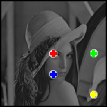
\includegraphics[width=\textwidth]{./figures/results/no_helix/rawinput_colour}
%     \caption{Raw input for OPT simulations, Lena.}
%     \label{fig:raw_input}
%   \end{subfigure}\hfill
%   \begin{subfigure}[t]{0.3\textwidth}
%     \includegraphics[width=\textwidth]{./figures/results/no_helix/sinogram_stretch}
%     \caption{Image of Lena (\figurename~\ref{fig:raw_input}) after rotation and projection in 2D, giving the sinogram.}
%     \label{fig:sinogram_stretch}
%   \end{subfigure}
%   \hfill
%   \label{fig:rawinputs}
%   \caption{Reference images for OPT reconstruction.}
% \end{figure}

\begin{figure}
    % \begin{subfigure}[t]{\linewidth}
        \centering
        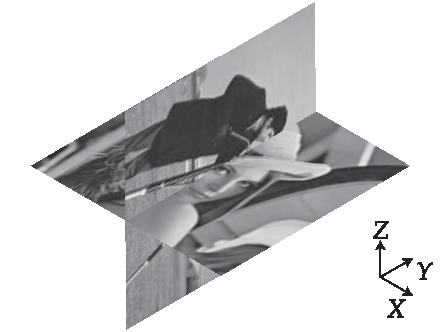
\includegraphics[width=0.4\textwidth]{./figures/ortho_3d_correct}
        \caption{Ground truth 3D object for reconstruction, based on the Cameraman and Lena testcard images.}\label{fig:ortho_3d_correct}
    % \end{subfigure}
\end{figure}
\begin{figure}
% \ContinuedFloat{}
    \begin{subfigure}[t]{0.2\linewidth}
        \centering
        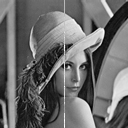
\includegraphics[width=\textwidth]{./figures/results/3D_python/no_drift/0/xy}\caption{Raw\\Frame (\(n\)): 0\\View: (\(X,Y\))}
    \end{subfigure}\hfill
    \begin{subfigure}[t]{0.2\linewidth}
        \centering
        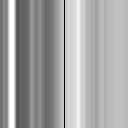
\includegraphics[width=\textwidth]{./figures/results/3D_python/no_drift/0/xy_recon}\caption{Reconstructed\\Frame (\(n\)): 0\\View: (\(X,Y\))}
    \end{subfigure}\hfill
    \begin{subfigure}[t]{0.2\linewidth}
        \centering
        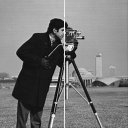
\includegraphics[width=\textwidth]{./figures/results/3D_python/no_drift/0/zx}\caption{Raw\\Frame (\(n\)): 0\\View: (\(Z,Y\))}
    \end{subfigure}\hfill
    \begin{subfigure}[t]{0.2\linewidth}
        \centering
        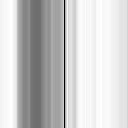
\includegraphics[width=\textwidth]{./figures/results/3D_python/no_drift/0/zx_recon}\caption{Reconstructed\\Frame (\(n\)): 0\\View: (\(Z,Y\))}
    \end{subfigure}
    \begin{subfigure}[t]{0.2\linewidth}
        \centering
        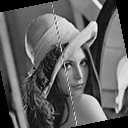
\includegraphics[width=\textwidth]{./figures/results/3D_python/no_drift/1/xy}\caption{Raw\\Frame (\(n\)): 1\\View: (\(X,Y\))}
    \end{subfigure}\hfill
    \begin{subfigure}[t]{0.2\linewidth}
        \centering
        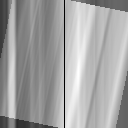
\includegraphics[width=\textwidth]{./figures/results/3D_python/no_drift/1/xy_recon}\caption{Reconstructed\\Frame (\(n\)): 1\\View: (\(X,Y\))}
    \end{subfigure}\hfill
    \begin{subfigure}[t]{0.2\linewidth}
        \centering
        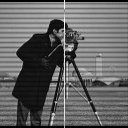
\includegraphics[width=\textwidth]{./figures/results/3D_python/no_drift/1/zx}\caption{Raw\\Frame (\(n\)): 1\\View: (\(Z,Y\))}
    \end{subfigure}\hfill
    \begin{subfigure}[t]{0.2\linewidth}
        \centering
        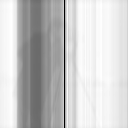
\includegraphics[width=\textwidth]{./figures/results/3D_python/no_drift/1/zx_recon}\caption{Reconstructed\\Frame (\(n\)): 1\\View: (\(Z,Y\))}
    \end{subfigure}
    \begin{subfigure}[t]{0.2\linewidth}
        \centering
        
\includegraphics[width=\textwidth]{./figures/results/3D_python/no_drift/dots/xy}%\caption{Raw data. Frame (\(n\)): , View: \(xy\)}
    \end{subfigure}\hfill
    \begin{subfigure}[t]{0.2\linewidth}
        \centering
        
\includegraphics[width=\textwidth]{./figures/results/3D_python/no_drift/dots/xy_recon}%\caption{Reconstructed\\Frame (\(n\)):0, View:\(xy\)}
    \end{subfigure}\hfill
    \begin{subfigure}[t]{0.2\linewidth}
        \centering
        
\includegraphics[width=\textwidth]{./figures/results/3D_python/no_drift/dots/zx}%\caption{Raw data. Frame (\(n\)): , View: \(zy\)}
    \end{subfigure}\hfill
    \begin{subfigure}[t]{0.2\linewidth}
        \centering
        
\includegraphics[width=\textwidth]{./figures/results/3D_python/no_drift/dots/zx}%\caption{Reconstructed\\Frame (\(n\)):, View:\(zx\)}
    \end{subfigure}
    \begin{subfigure}[t]{0.2\linewidth}
        \centering
        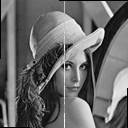
\includegraphics[width=\textwidth]{./figures/results/3D_python/no_drift/31/xy}\caption{Raw\\Frame (\(n\)): 31\\View: (\(X,Y\))}
    \end{subfigure}\hfill
    \begin{subfigure}[t]{0.2\linewidth}
        \centering
        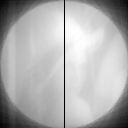
\includegraphics[width=\textwidth]{./figures/results/3D_python/no_drift/31/xy_recon}\caption{Reconstructed\\Frame (\(n\)): 31\\View: (\(X,Y\))}
    \end{subfigure}\hfill
    \begin{subfigure}[t]{0.2\linewidth}
        \centering
        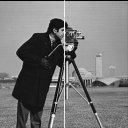
\includegraphics[width=\textwidth]{./figures/results/3D_python/no_drift/31/zx}\caption{Raw\\Frame (\(n\)): 31\\View: (\(Z,Y\))}
    \end{subfigure}\hfill
    \begin{subfigure}[t]{0.2\linewidth}
        \centering
        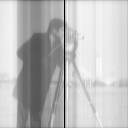
\includegraphics[width=\textwidth]{./figures/results/3D_python/no_drift/31/zx_recon}\caption{Reconstructed\\Frame (\(n\)): 31\\View: (\(Z,Y\))}
    \end{subfigure}
    \caption[A 3D test-volume of two orthogonal and different testcard images, was used to verify the reconstructive capabilities of the proposed algorithm]{
    A 3D test-volume of two orthogonal and different testcard images, from \figurename~\ref{fig:ortho_3d_correct}, was used to verify the reconstructive capabilities of the proposed algorithm.
    The projected image data (b),~(h),~(j) and (d),~(h),~(l), were used to iteratively generate reconstructions where the \(n^\text{th}\) reconstruction incorporates all the information from observation 0 to \(n\).
    The results are unfiltered for clarity of demonstrating the iterative reconstruction, which is applied in \figurename~\ref{fig:flopt_filter}.
    }\label{fig:recon_iterative}
    %TODO use different filters.
\end{figure}


In the standard approach for \gls{OPT} reconstruction, the sinogram undergoes the inverse \gls{Radon transform}, as shown in \figurename~\ref{fig:iradon_nofilter} and then post-filtering, see \figurename~\ref{fig:iradon_filter}.
This step is substituted for the proposed algorithm; in \figurename~\ref{fig:flopt_comparison_line_profile} the two techniques are compared for ideal conditions of smooth, predictable rotation.
The proposed algorithm produces %(see )
a faithful reconstruction on the original image, as shown in \figurename~\ref{fig:flopt_filter} %with some minor deviations.
Both techniques lose some of the original contrast of the object due to under-sampling of rotations.
When taking the histogram of the absolute pixel-wise difference between the original source image to the images produced by the new algorithm and the \gls{Radon transform},
% there is good overlap between the two,
see \figurename~\ref{fig:flopt_histogram}.
The mean square errors (\gls{MSE}, see Equation~\eqref{eq:mse}) of the new algorithm and the \gls{Radon transform} are \SI{15.01}{\percent} and \SI{14.84}{\percent} respectively, see \figurename~\ref{fig:flopt_histogram} for a histogram of a pixel-wise comparison.
This suggests that the new algorithm is producing an accurate reconstruction of the object, similar to the standard \gls{Radon transform}.
%, see \figurename~\ref{fig:flopt_histogram}

\begin{align}
    \operatorname{\gls{MSE}}=\frac{1}{n}\sum_{i=1}^n{(Y_i-\hat{Y_i})}^2 \label{eq:mse} % \intertext{Where \(\hat{Y_i}\) is the ith value and Y_i }
\end{align}

\begin{figure}
  \centering
  \begin{subfigure}[t]{0.45\textwidth}
    \centering
    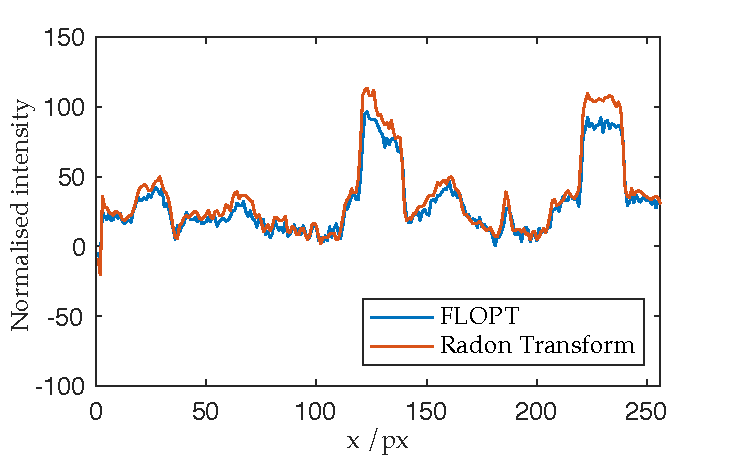
\includegraphics[width=\textwidth]{./figures/results/comparison_line_profile}
    % \caption[Line profile comparison of the standard and new algorithms]{Line profile comparison of the reconstruction of a reference image computationally rotated, projected and reconstructed using the standard \gls{Radon transform} and the new proposed algorithm.}
    \caption{}\label{fig:flopt_comparison_line_profile}
  \end{subfigure}\quad
 \begin{subfigure}[t]{0.45\textwidth}
    \centering
    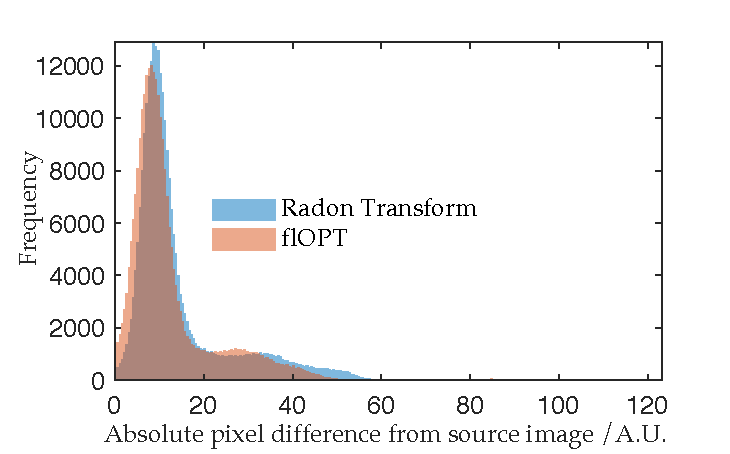
\includegraphics[width=\textwidth]{./figures/results/flopt_histogram}
    % \caption[Histogram of pixel values compared between reconstructions using flOPT and the \gls{Radon transform}]{Histogram of of pixel values compared between reconstructions using flOPT and the \gls{Radon transform}.
    % The shift of the histogram to towards overall lower deviance from the source image suggests the flOPT algorithm out performs the \gls{Radon transform}}\label{fig:flopt_histogram}
    \caption{}\label{fig:flopt_histogram}
  \end{subfigure}\\
  \begin{subfigure}[t]{0.45\textwidth}
    \centering
    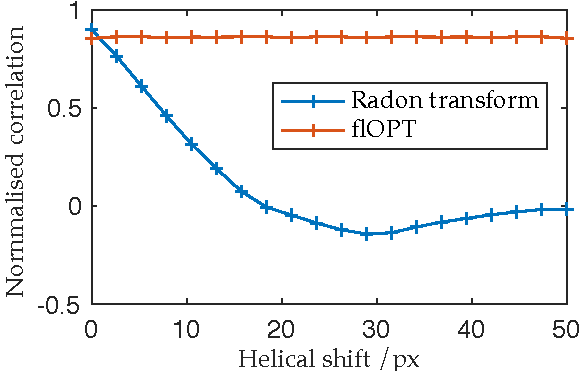
\includegraphics[width=\textwidth]{./figures/results/correlation_helicity}
    % \caption[Comparison of standard and proposed OPT reconstruction algorithms for acquisitions with drift]{%2D correlation of the source image shows that flOPT does not degrade under systematic drift compared to s.
    % Comparison of standard and proposed \gls{OPT} reconstruction algorithms for acquisitions with drift.
    % 2D image correlation of the ground truth and the reconstruction shows that the proposed flOPT algorithm does not degrade with systematic drift, whereas reconstruction using the standard \gls{Radon transform} is severely degraded.
    % }
    \caption{}\label{fig:helical_comparison}
  \end{subfigure}
  \caption{
  (\subref{fig:flopt_comparison_line_profile}), Line profile comparison of the reconstruction of a reference image computationally rotated, projected and reconstructed using the standard \gls{Radon transform} and the new proposed algorithm.
  (\subref{fig:flopt_histogram}), Histogram of of pixel values compared between reconstructions using flOPT and the \gls{Radon transform}.
  The shift of the histogram to towards overall lower deviance from the source image suggests the flOPT algorithm out performs the \gls{Radon transform}
  (\subref{fig:helical_comparison}): Comparison of standard and proposed \gls{OPT} reconstruction algorithms for acquisitions with drift.
  2D image correlation of the ground truth and the reconstruction shows that the proposed flOPT algorithm does not degrade with systematic drift, whereas reconstruction using the standard \gls{Radon transform} is severely degraded.}
\end{figure}

%However, the proposed algorithm fairs worse in terms of contrast compared to a \gls{Radon transform}.

The more challenging case of a sample drifting, with a constant velocity and systematically along the \(X\) axis was then considered; this produced a helical path of a single fiducial within the sample, see \figurename~\ref{fig:flopt_helix_sinogram}.
In \figurename~\ref{fig:unfilttered_reconstruction_helix_iradon}, the \gls{Radon transform} entirely fails to produce a recognisable reproduction of the test image with the addition of a slight helicity to the rotation.
The proposed algorithm produces an equivalent result to that of a sample rotating without any systematic drift, see \figurename~\ref{fig:iradon_filter}.
In \figurename~\ref{fig:helical_comparison} the respective images from each algorithm were compared, as before, while the helical shift was incremented.
See \figurename~\ref{fig:flopt_helix_sinogram} for a sinogram of a sample whereby a helical shift has been induced.
When using correlation as a metric of reproduction quality, at zero helicity, the new algorithm fairs slightly worse at \SI{94}{\percent} correlation compared to the \gls{Radon transform} at \SI{96}{\percent}.
As expected, the \gls{Radon transform} rapidly deteriorates once a systematic drift is applied; whereas the new algorithm maintains the quality of the reconstruction, see \figurename~\ref{fig:helical_comparison}.

\begin{figure}
  \centering
  \hspace*{\fill}
 \begin{subfigure}[t]{0.3\textwidth}
   \begin{tikzpicture}[node distance=0cm]
     \node (img) {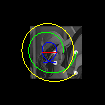
\includegraphics[width=0.8\textwidth]{./figures/results/helix/topdown_bead_paths}};
      \node[below=of img] {\(X\)};
      \node[left=of img,rotate=90,yshift=0.2cm] {\(Y\)};
   \end{tikzpicture}
   \caption{Top down views (\(X,Y\)) of the source image with the fiducial paths marked.}\label{fig:topdown_bead_paths}
 \end{subfigure}\hfill
 \begin{subfigure}[t]{0.3\textwidth}
   \begin{tikzpicture}[node distance=0cm]
     \node (img) {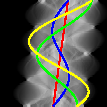
\includegraphics[width=0.8\textwidth]{./figures/results/helix/sinugram_stretch}};
      \node[below=of img] {\(v\)\vphantom{\(X\)}};
      \node[left=of img,rotate=90,yshift=0.2cm] {\(n\)};
   \end{tikzpicture}
   \caption{Sinogram (\(v,n\)) of a sample whose axis of rotation has a systematic drift}\label{fig:flopt_helix_sinugram}
 \end{subfigure}\hspace*{\fill}
  \\\vspace{\abovecaptionskip}
  \hspace*{\fill}
  \begin{subfigure}[t]{0.3\textwidth}
    \begin{tikzpicture}[node distance=0cm]
      \node (img) {
\includegraphics[width=0.8\textwidth]{./figures/results/helix/unfilttered_reconstruction_helix_iradon}};
       \node[below=of img] {\(X\)};
       \node[left=of img,rotate=90,yshift=0.2cm] {\(Y\)};
    \end{tikzpicture}
    \caption{Unfiltered reconstruction using a \gls{Radon transform}.}\label{fig:unfilttered_reconstruction_helix_iradon}
  \end{subfigure}\hfill
  \begin{subfigure}[t]{0.3\textwidth}
    \begin{tikzpicture}[node distance=0cm]
      \node (img1) {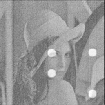
\includegraphics[width=0.8\textwidth]{./figures/results/helix/filtered_recon_helix}};
       \node[below=of img1] {\(v\)\vphantom{\(X\)}};
       \node[left=of img1,rotate=90,yshift=0.2cm] {\(Y\)};
    \end{tikzpicture}
    \caption{Filtered reconstruction using the new algorithm.}\label{fig:filtered_recon_helix}
  \end{subfigure}
   \hspace*{\fill}
   % \caption{}
  \caption{Comparison of the two reconstructions under sample imaging with a systematic drift, in 3D though represented here in 2D.}\label{fig:flopts}
\end{figure}

\subsection{Recovery of R and T using matrix decomposition}

To quantitatively verify that the matrix decomposition technique was valid and robust, the accuracy of the reproduction of \gls{R} and \gls{T} was tested directly.
The original \gls{R} and \gls{T} matrices were computed and compared to \gls{R} and \gls{T} generated from matrix decomposition, this absolute difference was computed element-wise in each matrix and then an average for each matrix was taken.
Overall, the worst case scenario produced a percentage error of \SI{2}{\percent} (see \figurename~\ref{fig:pc_sum_decompose} for full statistics).
The accuracy of the calculated \gls{R} and \gls{T} did deteriorate when adding in additional degrees of combined movement, but with no correlation between the degree of helicity and the error produced.
% but the severity of this movement appeared to no trending effect.
Consistently the translational matrix (\gls{T}) was more accurately reproduced, this is likely due to there being fewer of degrees of freedom for errors to spread over.

%The images produced are a more faithful reproduction of the source image as the degree of helicity is increased.
%This effect may be due to the additional sampling induced by adding another degree of movement, that is the systematic drift.

%Textwidth is \the\textwidth


\begin{figure}
  \centering
    \begin{subfigure}[t]{0.5\textwidth}
      \captionsetup{width=0.8\textwidth}
      \centering
      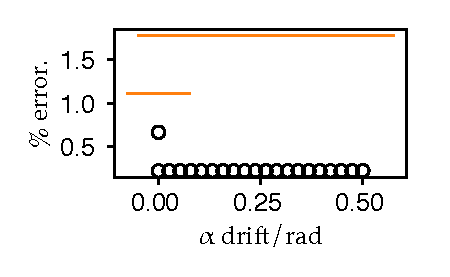
\includegraphics[width=\textwidth]{./figures/results/helix/decompose/pc_sum_rot_alpha}
      \caption{Rotation matrix, with angular drift in \(\alpha \)}\label{fig:pc_sum_rot_alpha}
    \end{subfigure}\hfill
    \begin{subfigure}[t]{0.5\textwidth}
      \captionsetup{width=0.8\textwidth}
      \centering
      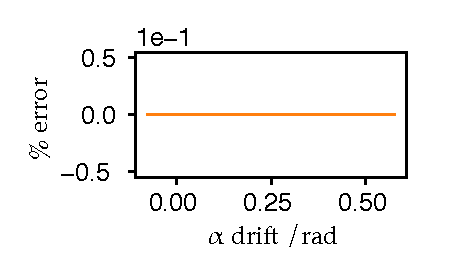
\includegraphics[width=\textwidth]{./figures/results/helix/decompose/pc_sum_trans_alpha}
      \caption{Translation matrix, with angular drift in \(\alpha \)}\label{fig:pc_sum_trans_alpha}
    \end{subfigure}
    \bigskip
        \begin{subfigure}[t]{0.5\textwidth}
          \captionsetup{width=0.8\textwidth}
          \centering
          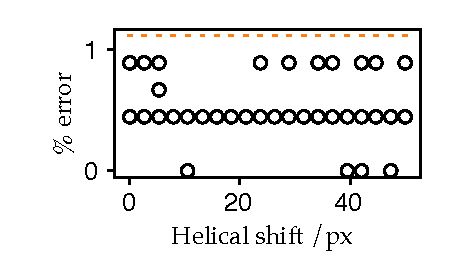
\includegraphics[width=\textwidth]{./figures/results/helix/decompose/pc_sum_rot_tx}
          \caption{Rotation matrix, with helical drift in \(x\) only}\label{fig:pc_sum_rot_tx}
        \end{subfigure}\hfill
        \begin{subfigure}[t]{0.5\textwidth}
          \captionsetup{width=0.8\textwidth}
          \centering
          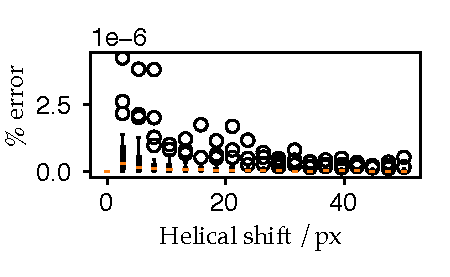
\includegraphics[width=\textwidth]{./figures/results/helix/decompose/pc_sum_trans_tx}
          \caption{Translation matrix, with helical drift in \(x\) only}\label{fig:pc_sum_trans_tx}
        \end{subfigure}
    \bigskip
        \begin{subfigure}[t]{0.5\textwidth}
          \captionsetup{width=0.8\textwidth}
          \centering
          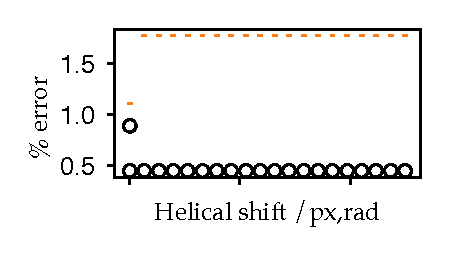
\includegraphics[width=\textwidth]{./figures/results/helix/decompose/pc_sum_rot_both}
          \caption{Rotation matrix, with angular drift in \(\alpha \) and helical drift in \(x\)}\label{fig:pc_sum_rot_both}
        \end{subfigure}\hfill
        \begin{subfigure}[t]{0.5\textwidth}
          \captionsetup{width=0.8\textwidth}
          \centering
          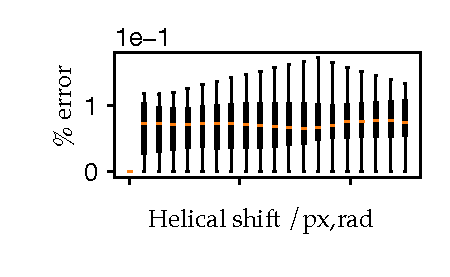
\includegraphics[width=\textwidth]{./figures/results/helix/decompose/pc_sum_trans_both}
          \caption{Translation matrix, with angular drift in \(\alpha \) and helical drift in \(X\)}\label{fig:pc_sum_trans_both}
        \end{subfigure}
          \caption[Box plots demonstrating that the rotational and translations matrices can be recovered accurately from fiducial marker positions]{Box plots demonstrating that the rotational and translations matrices can be recovered accurately from fiducial marker positions.
          Panels~(\subref{fig:pc_sum_rot_alpha}) and~(\subref{fig:pc_sum_trans_alpha}) introduce an angular drift during rotation, to an observer at the detector this would appear as a tip of the sample towards them, causing precession.
          Panels~(\subref{fig:pc_sum_rot_tx}) and~(\subref{fig:pc_sum_trans_tx}) introduce a lateral drift in \(X\) causing a helical path to be drawn out.
          Panels~(\subref{fig:pc_sum_rot_both}) and~(\subref{fig:pc_sum_trans_both}) combine the two effects.
          In all cases the percentage error introduced by the the addition of undesirable additional movements was on the order of \SI{<2}{\percent}.
          }\label{fig:pc_sum_decompose}
\end{figure}

\section{Discussion}

A new algorithm for reconstructing OPT data has been demonstrated.
The new algorithm uses multiple fiducial markers to recover the matrix which describes the rotation and translation of the sample.
The quality of the reconstructions when compared to the standard \gls{Radon transform} shows a slight improvement, with a great effect when a systematic drift is introduced.
The accuracy of the decomposition of \gls{F} into \gls{R} and \gls{T} were compared to the ground truth matrices.
The element-wise absolute difference \(\left(\frac{x-y}{2(x+y)}\right)\) of each matrix was averaged across the matrix for \gls{R} and \gls{T}.
In the worst case scenario a maximum of \SI{2}{\percent} average absolute difference was found between ground truth and recovered matrices,
% When comparing the
% expected matrices to the recovered matrices a
% ground truth matrices to the recovered matrices were compared using the average of the element-wise using square differences
% peak of \SI{2}{\percent} difference is found between the two when considering worst case scenarios;
suggesting the technique is robust to various forms of drift and general instability.
Such an algorithm could be used to help in minimising ghosting effects seen in real samples; particularly in samples where slipping is likely to occur such as in gels or in cheaper \gls{OPT} systems which tend to be more mechanically unstable and imprecise.

\section{Future work}

The theory backing the proposed algorithm relies on triangulation between two view points.
% In this work the two view points refer to the image at frames \(n\) and \(n+1\).
However, it is possible to use three separate views %(frames \(n\), \(n+1\) and \(n+2\))
to reconstruct a scene, one such approach being quaternion tensors.
Working with tensors is more complex, but a future iteration of the algorithm presented here may benefit from using three views to provide a more accurate transformation matrix.
Beyond three views there currently is no mathematical framework at present for four or more views.
If such tools did exist, it may be possible to have the algorithm described above be a non-iterative and essentially a single shot reconstruction from pixels to voxels.

% In computer vision, scenes often do not contain known fiducial marks and so such marks are found between views.
Fiducial markers could also be extracted from the image texture alone, circumventing the need for for the additional beads embedded in the sample.
To find such a correspondences, points with similar local texture are found and matched in between each image using standard algorithms such as SIFT~\cite{} and RANSAC\cite{}. %, many of these such correspondences are found
This was attempted however the errors introduced into the transformation matrices appear to make the approach currently untenable.
% This technique is only valid for views with small angles between them, as would be found in \gls{OPT}.

\pagebreak

\section{Introduction}
Adherence to the specifications listed in this template is essential for efficient review and publication of submissions. Proper reference format is especially important (see Section \ref{sec:refs}).

\section{Multiple corresponding authors}

There are two options for indicating multiple corresponding authorship, and they are formatted quite differently. The first format would be as follows and uses an asterisk to denote one of the authors:

\begin{verbatim}
\author{Author One\authormark{1,3} and Author Two\authormark{2,4,*}}

\address{\authormark{1}Peer Review, Publications Department,
Optical Society of America, 2010 Massachusetts Avenue NW,
Washington, DC 20036, USA\\
\authormark{2}Publications Department, Optical Society of America,
2010 Massachusetts Avenue NW, Washington, DC 20036, USA\\
\authormark{3}xyz@osa.org}

\email{\authormark{*}opex@osa.org}
\end{verbatim}

This format will generate the following appearance:

\medskip

\author{Author One\authormark{1,3} and Author Two\authormark{2,4,*}}

\address{\authormark{1}Peer Review, Publications Department,
Optical Society of America, 2010 Massachusetts Avenue NW,
Washington, DC 20036, USA\\
\authormark{2}Publications Department, Optical Society of America,
2010 Massachusetts Avenue NW, Washington, DC 20036, USA\\
\authormark{3}xyz@osa.org}

\email{\authormark{*}opex@osa.org}

\medskip

The second format forgoes the asterisk and sets all email addresses equally within the affiliations. Please note that this format does not use the \verb+\email{}+ field at all.
\begin{verbatim}
\author{Author One\authormark{1,3} and Author Two\authormark{2,4}}

\address{\authormark{1}Peer Review, Publications Department,
Optical Society of America, 2010 Massachusetts Avenue NW,
Washington, DC 20036, USA\\
\authormark{2}Publications Department, Optical Society of America,
2010 Massachusetts Avenue NW, Washington, DC 20036, USA\\
\authormark{3}xyz@osa.org\\
\authormark{4}opex@osa.org}
\end{verbatim}

This format will generate the following appearance:

\medskip

\author{Author One\authormark{1,3} and Author Two\authormark{2,4}}

\address{\authormark{1}Peer Review, Publications Department,
Optical Society of America, 2010 Massachusetts Avenue NW, Washington, DC 20036, USA\\
\authormark{2}Publications Department, Optical Society of America, 2010 Massachusetts Avenue NW, Washington, DC 20036, USA\\
\authormark{3}xyz@osa.org\\
\authormark{4}opex@osa.org}
\medskip
These are the preferred
%express journal
formats for multiple corresponding authorship, and either may be used.


The abstract should be limited to approximately 100 words.
%It should be an explicit summary of the paper that states the problem, the methods used, and the major results and conclusions. It also should contain the relevant key words that would allow it to be found in a cursory computerized search.
If the work of another author is cited in the abstract, that citation should be written out without a number, (e.g., journal, volume, first page, and year in square brackets [Opt. Express {\bfseries 22}, 1234 (2014)]), and a separate citation should be included in the body of the text. The first reference cited in the main text must be [1]. Do not include numbers, bullets, or lists inside the abstract.

\begin{figure}[h!]
\centering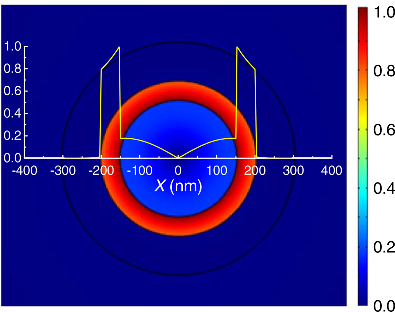
\includegraphics[width=7cm]{osafig1}
\caption{Sample caption (Fig. 2, \cite{Yelin:03}).}
\end{figure}


\section{Assessing final manuscript length}
OSA's Universal Manuscript Template is based on the OSA Express layout and will provide an accurate length estimate for Optics Express, Biomedical Optics Express,  Optical Materials Express, and OSA's newest title OSA Continuum. Applied Optics, JOSAA, JOSAB, Optics Letters, Optica, and Photonics Research publish articles in a two-column layout. To estimate the final page count in a two-column layout, multiply the manuscript page count (in increments of 1/4 page) by 60\%. For example, 11.5 pages in the OSA Universal Manuscript Template are roughly equivalent to 7 composed two-column pages. Note that the estimate is only an approximation, as treatment of figure sizing, equation display, and other aspects can vary greatly across manuscripts. Authors of Letters may use the legacy template for a more accurate length estimate.

\section{Figures, tables, and supplemental materials}

\subsection{Figures and tables}

OSA encourages authors to submit color figures with their manuscripts. Figures and tables should be placed in the body of the manuscript. Standard \LaTeX{} environments should be used to place tables and figures:
\begin{verbatim}
\begin{figure}[htbp]
\centering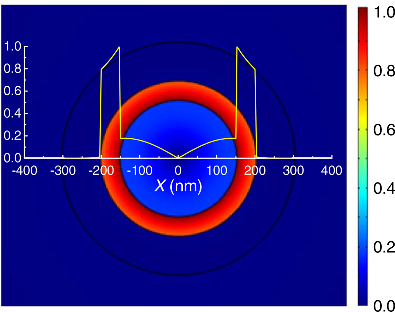
\includegraphics[width=7cm]{osafig1}
\caption{Sample caption (Fig. 2, \cite{Yelin:03}).}
\end{figure}
\end{verbatim}

\subsection{Supplementary materials in OSA journals}

OSA journals allow authors to include supplementary materials as integral parts of a manuscript. Such materials are subject to peer-review procedures along with the rest of the paper and should be uploaded and described using OSA's Prism manuscript system. Please see the \href{http://www.osapublishing.org/submit/style/multimedia.cfm}{Author Guidelines for Supplementary Materials in OSA Journals} for further information.

Supplementary materials must be associated with a figure, table, or equation, OR be referenced in the results section of the manuscript. Please note that to create text color for supplementary materials links, use of the command \\
\verb|\textcolor{urlblue}{Visualization 1}| is preferred to using the command\\
\verb|\url{Visualization 1}|.

\begin{figure}[ht!]
\centering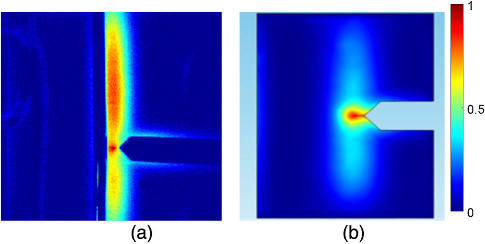
\includegraphics{osafig2}
\caption{(a) Three traps create three rings of magnetic nanoparticles. (b) The rings interact with one another (see \textcolor{urlblue}{Visualization 1}, \cite{Masajada:13}).}
\end{figure}


\begin{verbatim}
\begin{figure}[hbt!]
\centering\includegraphics{opexfig2}
\caption{Normalized modulus distributions of transverse electrical
field components of the TM01 mode in PWs with (a) SiO_2 core
and (b) Si core}{Visualization 1}), \cite{Masajada:13}).}
\end{figure}
\end{verbatim}

\section{Mathematical and scientific notation}

\subsection{Displayed equations} Displayed equations should be centered.
Equation numbers should appear at the right-hand margin, in
parentheses:
\begin{equation}
J(\rho) =
 \frac{\gamma^2}{2} \; \sum_{k({\rm even}) = -\infty}^{\infty}
	\frac{(1 + k \tau)}{ \left[ (1 + k \tau)^2 + (\gamma  \rho)^2  \right]^{3/2} }.
\end{equation}

All equations should be numbered in the order in which they appear
and should be referenced  from within the main text as Eq. (1),
Eq. (2), and so on [or as inequality (1), etc., as appropriate].


\section*{Funding}
Please identify all appropriate funding sources by name and contract number. Funding information should be listed in a separate block preceding any acknowledgments. List only the funding agencies and any associated grants or project numbers, as shown in the example below:\\
\\
National Science Foundation (NSF) (1253236, 0868895, 1222301); Program 973 (2014AA014402); Natural National Science Foundation (NSFC) (123456).\\
\\
OSA participates in \href{https://www.crossref.org/fundingdata/}{Crossref's Funding Data}, a service that provides a standard way to report funding sources for published scholarly research. To ensure consistency, please enter any funding agencies and contract numbers from the Funding section in Prism during submission or revisions.

\section*{Acknowledgments}
Acknowledgments, if included, should appear at the end of the document. The section title should not be numbered.

\section*{Disclosures}
For \textit{Biomedical Optics Express} submissions only, disclosures should be listed in a separate nonnumbered section at the end of the manuscript. List the Disclosures codes identified on OSA's \href{http://www.osapublishing.org/submit/review/conflicts-interest-policy.cfm}{Conflict of Interest policy page}, as shown in the examples below:\\
\\
ABC: 123 Corporation (I,E,P), DEF: 456 Corporation (R,S). GHI: 789 Corporation (C).\\
\\
If there are no disclosures, then list ``The authors declare that there are no conflicts of interest related to this article.''


\section{References}
\label{sec:refs}
Proper formatting of references is extremely important, not only for consistent appearance but also for accurate electronic tagging. Please follow the guidelines provided below on formatting, callouts, and use of Bib\TeX.

\subsection{Formatting reference items}
Each source must have its own reference number. Footnotes (notes at the bottom of text pages) are not used in OSA journals. References require all author names, full titles, and inclusive pagination. Examples of common reference types can be found on the  \href{http://www.osapublishing.org/submit/style/style_traditional_journals.cfm} {Author and Reviewer Resource Center}.


The commands \verb+\begin{thebibliography}{}+ and \verb+\end{thebibliography}+ format the section according to standard style, showing the title {\bfseries References}.  Use the \verb+\bibitem{label}+ command to start each reference.

\subsection{Formatting reference citations}
References should be numbered consecutively in the order in which they are referenced in the body of the paper. Set reference callouts with standard \verb+\cite{}+ command or set manually inside square brackets [1].

To reference multiple articles at once, simply use a comma to separate the reference labels, e.g. \verb+\cite{Yelin:03,Masajada:13,Zhang:14}+, produces \cite{Yelin:03,Masajada:13,Zhang:14}.
%Using the \texttt{cite.sty} package will make these citations appear like so: [2--4].

\subsection{Bib\TeX}
\label{sec:bibtex}
Bib\TeX{} may be used to create a file containing the references, whose contents (i.e., contents of \texttt{.bbl} file) can then be pasted into the bibliography section of the \texttt{.tex} file. A Bib\TeX{} style file, \texttt{osajnl.bst}, is provided.

\section{Conclusion}
After proofreading the manuscript, compress your .tex manuscript file and all figures (which should be in EPS or PDF format) in a ZIP, TAR or TAR-GZIP package. All files must be referenced at the root level (e.g., file \texttt{figure-1.eps}, not \texttt{/myfigs/figure-1.eps}). If there are supplementary materials, the associated files should not be included in your manuscript archive but be uploaded separately through the Prism interface.

%%%%%%%%%%%%%%%%%%%%%%% References %%%%%%%%%%%%%%%%%%%%%%%%%

Add references with BibTeX or manually.
\cite{Zhang:14,OSA,FORSTER2007,Dean2006}

%%%%%%%%%% If using BibTeX:
\bibliography{sample}

%%%%%%%%%% If preparing manually:
% \begin{thebibliography}{1}
% \newcommand{\enquote}[1]{``#1''}

% \bibitem{Zhang:14}
% Y.~Zhang, S.~Qiao, L.~Sun, Q.~W. Shi, W.~Huang, L.~Li, and Z.~Yang,
%   \enquote{Photoinduced active terahertz metamaterials with nanostructured
%   vanadium dioxide film deposited by sol-gel method,}
%   {\protect\JournalTitle{Optics Express}} \textbf{22}, 11070--11078 (2014).

% \bibitem{OSA}
% {Optical Society}, \enquote{{OSA Publishing},}
%   \url{http://www.osapublishing.org}.

% \bibitem{FORSTER2007}
% P.~Forster, V.~Ramaswamy, P.~Artaxo, T.~Bernsten, R.~Betts, D.~Fahey,
%   J.~Haywood, J.~Lean, D.~Lowe, G.~Myhre, J.~Nganga, R.~Prinn, G.~Raga,
%   M.~Schulz, and R.~V. Dorland, \enquote{Changes in atmospheric consituents and
%   in radiative forcing,} in \enquote{Climate Change 2007: The Physical Science
%   Basis. Contribution of Working Group 1 to the Fourth assesment report of
%   Intergovernmental Panel on Climate Change,}  S.~Solomon, D.~Qin, M.~Manning,
%   Z.~Chen, M.~Marquis, K.~B. Averyt, M.~Tignor, and H.~L. Miler, eds.
%   (Cambridge University Press, 2007).

% \end{thebibliography}

\pagebreak
\section{Supplemental}
\subsection{Reconstruction}

As the sample is rotated each detector pixel collects an intensity \(I(\theta) = I_{n}e^{-k(\theta)}\) at discrete (\(n\)) angles through a full rotation of the sample; where \(I_{n}\) is the unattenuated radiation intensity from the source to the detector, \(k\) is the attenuation caused by the sample along a detected ray an \(I(n)\) is the measured intensity, see \figurename~\ref{fig:OPT_digram}.
Rays from the sample to the detector approximate straight lines, and so the the rays reaching the detector with a line integrals.
A projection is then the resulting intensity profile at the detector for a rotation angle, and the integral transform that results in \(P_\theta(v)\)
% \(f(I_i,\theta_n) \)
is the \gls{Radon transform}.
% This is defined mathematically as:

\begin{align}
    \intertext{The equation of a set of parallel rays from a source passing through the specimen to a point \(v\) along the detector is:}
    &X\cos(\theta) + Y\sin(\theta) - v = 0 \\
    \intertext{Projecting many such rays through a sample with structure \(f(X,Y)\) gives:}
    P_\theta(v) = &\int_{\infty}^{\infty} \int_{\infty}^{\infty} f(X,Y)\delta (x\cos(\theta)+y \sin(\theta)-v)dX dY
\end{align}

% \begin{figure}
%     \centering
%     \includegraphics{coordinate_system}
%     \caption{Coordinate system}
%     \label{fig:coordinate_system_flopt}
% \end{figure}

Where \(P_\theta(v)\) is the \gls{Radon transform} of \(f(X,Y)\) which represents the contrast image of \gls{2D} slice of the specimen.
The \gls{Radon transform} of an image produces a \gls{sinugram} as in \figurename~\ref{fig:rawinputs}


% A parallel projection is then just the combination of line integrals  \(f(I) \) for a constant. % for a constant.

An inverse \gls{Radon transform} is used to recover the original object from the projection data; which is achieved by taking the \gls{Fourier transform} of each projection measurement, then reordering the information from the sample into the respective position in Fourier space.
This is valid due to the Fourier Slice theorem~\cite{bracewellStripIntegrationRadio1956} (see Appendix~\ref{appendix:fourierslice} for a derivation), which states that the \gls{Fourier transform} of a parallel projection is equivalent to a 2D slice of the Fourier transform of the original sample.
%A high pass filter such as a ramp filter is commonly used to counter the blurring caused by this oversampling.
% \gls{FBP} can be thought of as smearing the projection data across the image plane, and is expressed in equation form as:
\begin{align}
f_{\text{fpb}}(X,Y) = \int_{0}^{\pi} Q_\theta (X\cos(\theta)+Y\sin(\theta),\theta)dXdY
\end{align}

Where \(Q_\theta \) is the filtered projection data, and \(f_{\text{fpb}}(X,Y)\) is the back-projected image.
A spatial filtering step is applied during back-projection to avoid spatial frequency oversampling during the object’s rotation (see \figurename~\ref{fig:iradon_filter})
a high pass filter is commonly used to compensate for the perceived blurring.
The blurring arises as \(Q_\theta \) is back-projected (smeared) across the image plane for each angle of reconstruction; which means that not only does the back-projection contribute at the line it is intended to (along line \(C\) in \figurename~\ref{fig:coordinate_system_flopt}), but all other points along the back-projecting ray.
% The blurring occurs as \(Q_\theta\) makes the same contribution to the reconstruction for each angle
% will make the same contribution to the reconstruction at all of these points. Therefore, one could say that in the reconstruction process each filtered projection, Qe, is smeared back, or backprojected, over the image plane.


Now, suppose we know the relative positions of the two cameras and their respective intrinsic parameters, such as magnification and pixel offset.
For a single camera and given the camera parameters, we can translate pixel coordinates, \(\gls{w} = (u, v)\), into the coplanar image plane coordinates \(\gls{x}=(x, y)\):

\begin{align}
    u &= u_0 + k_u x \\
    v &= v_0 + k_v y
\end{align}

Knowing the focal length (\(f\)) of the imaging system, image plane coordinates may be projected into a ray in 3D.
The ray can be defined by using the point \gls{p} in camera-centred coordinates, where it crosses the image plane.

\begin{align}
  \mathbf{p} = \begin{bmatrix}
        x\\y\\z
      \end{bmatrix}
\end{align}

From the definition of a world point, as observed through an image, we can construct a dual-view model of world points in space as in \figurename~\ref{fig:epi-polar-geom}.
Using a model of a system with two views allows for the triangulation of rays based on image correspondences, this is an important part of stereo-vision.
The most important matching constraint which can be used the \emph{epipolar constraint}, and follows directly from the fact that the rays must intersect in 3D space.
Epipolar constraints facilitate the search for correspondences, they constrain the search to a 1D line in each image.
To derive general epipolar constraints, one should consider the epipolar geometry of two cameras as seen in \figurename~\ref{fig:epi-polar-geom}


The \textbf{baseline} is defined as the line joining the optical centres.
An \textbf{epipole} is the point of intersection of the baseline with the image plan and there are two epipoles per feature, one for each camera.
An \textbf{epipolar line} is a line of intersection of the epipolar plane with an image plane.
It is the image in one camera of the ray from the other camera’s optical centre to the world point (\gls{X}).
For different world points, the epipolar plane rotates about the baseline.
All epipolar lines intersect the epipole.

The epipolar line constrains the search for correspondence from a region to a line.
If a point feature is observed at \gls{x} in one image frame, then its location \gls{x'} in the other image frame must lie on the epipolar line.
We can derive an expression for the epipolar line.
The two camera-centered coordinate systems \gls{X_c'} and \gls{X_c} are related by a rotation, \gls{R} and translation, \gls{T} (see in \figurename~\ref{fig:epi-polar-geom}) as follows:

\begin{align}
    \gls{X_c'} &= \gls{R}\gls{X_c'} + \gls{T}
\end{align}
%       \\
%     \intertext{Taking the vector product with \(\gls{T}\), we obtain}
%     \gls{T} \times \gls{X_c'} &= \gls{T} \times \gls{R}\gls{X_c}+ \gls{T} \times \gls{T}  \\
%     \gls{T} \times \gls{X_c'} &= \gls{T} \times \gls{R}\gls{X_c}\label{eq:Xprime = RTX}
% \end{align}

% \begin{figure}
%   \centering
%   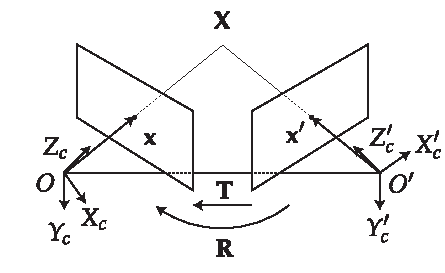
\includegraphics{./figures/epi-polar-geom}
%   \caption[Epi-polar geometry described for two adjacent views]{
%   Epi-polar geometry described for two adjacent views (or cameras of a scene).
%   Coordinates as expressed in \figurename~\ref{fig:coordinate_system_flopt} with prime notation (\('\)) denoting the additional right camera view.
%   Transforming from right to left camera-centered coordinates (\gls{X_c'} to \gls{X_c}) requires a rotation (\gls{R}) and a translation (\gls{T}).
%   }\label{fig:epi-polar-geom}
% \end{figure}

\subsection{The Essential matrix}

Taking the scalar product of \eqref{eq:Xprime = RTX} with \(\gls{X_c'}\), we obtain:
\begin{align}
    \gls{X_c'} \cdot (\gls{T} \times \gls{X_c}) &= \gls{X_c'}\cdot (\gls{T} \times \gls{R} \gls{X_c'}) \\
    \gls{X_c'} \cdot (\gls{T} \times \gls{R} \gls{X_c}) &= 0
    \intertext{A vector product can be expressed as a matrix multiplication:}
    \gls{T} \times \gls{X_c} &= \gls{T_x} \gls{X_c}
    \intertext{where}
    \gls{T_x} &=\begin{bmatrix}
    0    & -T_z  & T_y\\
    T_z  & 0     & -T_x\\
    -T_y  & T_x   & 0
    \end{bmatrix}
\end{align}
So equation~\eqref{eq:Xprime = RTX} can be rewritten as:

\begin{align}
\gls{X_c'} \cdot (\gls{T_x} \gls{R}\gls{X_c}) = 0 \\
\gls{X_c'} \gls{T} \gls{Essential} \gls{X_c}= 0 \\
\intertext{where}
\gls{Essential} = \gls{T_x} \gls{R}
\end{align}

\gls{Essential} is a \(3 \times 3\) matrix known as the \emph{essential matrix}.
The constraint also holds for rays \gls{p}, which are parallel to the camera-centered position vectors \gls{X_c}:

\begin{align}
\gls{p'}^T \gls{Essential} \gls{p} = 0 \label{eq:pEp}
\end{align}
This is the epipolar constraint.
If a point \gls{p} is observed in one image, then its position \gls{p'} in the other image must lie on the line defined by Equation~\eqref{eq:pEp}.
The essential matrix can convert from pixels on the detector to rays \gls{p} in the world, assuming a calibrated camera (intrinsic properties are known), and pixel coordinates can then be converted to image plane coordinates using:
\begin{align}
\begin{bmatrix}
u\\
v\\
1
\end{bmatrix}
&=
\begin{bmatrix}
k_u & 0 & u_0 \\
0 & k_v & v_0 \\
0 & 0 & 1
\end{bmatrix}
\begin{bmatrix}
x\\
y\\
1
\end{bmatrix}
\intertext{We can modify this to derive a relationship between pixel coordinates and rays:}
\begin{bmatrix}
u\\
v\\
1
\end{bmatrix}
&=
\begin{bmatrix}
\frac{k_u}{f} & 0 & \frac{u_0}{f} \\
0 & \frac{k_v}{f} & \frac{v_0}{f} \\
0 & 0 & \frac{1}{f}
\end{bmatrix}
\begin{bmatrix}
x\\
y\\
f
\end{bmatrix}
\intertext{\(\widetilde{\gls{K}}\) is defined as follows:}
\widetilde{\gls{K}} &= \begin{bmatrix}
f k_u & 0 & u_0 \\
0 & f k_v & v_0 \\
0 & 0 & 1
\end{bmatrix}
\intertext{then we can write pixel coordinates in homogenous coordinates:}
\widetilde{\gls{w}} &= \widetilde{\gls{K}} \gls{p}
\end{align}

\subsection{The Fundamental matrix}

\begin{align}
    \intertext{From~\eqref{eq:pEp} the epipolar constraint becomes}
    % \mathbf{p'}^T E \mathbf{p} &= 0 \\
    \widetilde{\gls{w'}} ^T \widetilde{\gls{K}}^{-T} E \widetilde{\gls{K}}^{-1} \widetilde{\gls{w}}  &= 0 \\
    \widetilde{\gls{w'}} ^T F \widetilde{\gls{w}}  &= 0
\end{align}
%\subsubsection{Two views}
%\paragraph{Mapping from one camera to another}
%\subsubsection{Three and more views}
The (\(3\times3)\) matrix \gls{F}, is the called the \emph{fundamental matrix}.
With intrinsically calibrated cameras, structure can be recovered by triangulation.
First, the two projection matrices are obtained via a \gls{SVD} of the essential matrix.
The \gls{SVD} of the essential matrix is given by:

\begin{align}
    \gls{Essential} &= \gls{K'}^T \gls{F} \gls{K} = \gls{T_x} \gls{R} = \mathbf{U}\Lambda \mathbf{V}^T\\%\gls{R} = U\LambdaV^T\\
    \intertext{It can be shown that}
    \hat{\gls{T_x}} &= U \begin{bmatrix}
    0 & 1 & 0 \\
    -1 & 0 & 0 \\
    0 & 0 & 0
    \end{bmatrix} U^T
    \intertext{ and }
    \gls{R} &= U \begin{bmatrix}
    0 & -1 & 0 \\
    1 & 0 & 0 \\
    0 & 0 & 1
    \end{bmatrix} V^T
    \intertext{Then, aligning the left camera and world coordinate systems gives the projection matrices:}
    \mathbf{P} &= \gls{K}    \begin{bmatrix}[c|c]       \mathbf{I} & \mathbf{0}   \end{bmatrix}
    \intertext{ and }
    \mathbf{P}' &= \gls{K'} \begin{bmatrix}[c|c]       \gls{R} & \gls{T}   \end{bmatrix}
\end{align}
Where \( \begin{bmatrix}[c|c] \mathbf{I} & \mathbf{0} \end{bmatrix}\) is the identity matrix augmented column-wise with a zero matrix, and the two projection matrices (\(\mathbf{P}\) and \(\mathbf{P}'\)) project from camera pixel coordinates to world coordinates.
Given these projection matrices, scene structure can be recovered (only up to scale, since only the magnitude of \gls{T} (|\gls{T}|) is unknown) using least squares fitting.
Ambiguities in \gls{T} and \gls{R} are resolved by ensuring that visible points lie in front of the two cameras.
As with the essential matrix, the fundamental matrix can be factorised into a skew-symmetric matrix corresponding
to translation and a \(3 \times 3\) non-singular matrix corresponding to rotation.


%
% \begin{figure}
%   \centering
%    \hspace*{\fill}
%   \begin{subfigure}[t]{0.3\textwidth}
%     
\includegraphics[width=\textwidth]{./figures/results/no_helix/iradon_nofilter}
%     \caption[Unfiltered iRadon]{This is the unfiltered reconstruction of the object using the \gls{Radon transform}}%TODO equation???
%     \label{fig:iradon_nofilter}
%   \end{subfigure}\hfill
%   \begin{subfigure}[t]{0.3\textwidth}
%     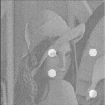
\includegraphics[width=\textwidth]{./figures/results/no_helix/iradon_filter}
%     \caption[Filtered iRadon]{Ram-lak (Fourier ramp) filter applied to \figurename~\ref{fig:iradon_nofilter}.}
%     \label{fig:iradon_filter}
%   \end{subfigure}
%      \hspace*{\fill}
%     % \label{fig:irandons}
%   \caption{The result of a tomographic reconstruction (using equally spaced angular steps and no translation between frames) requires Fourier filtering to normalise spatial contrast.}\label{fig:irandons}%TODO simulations with no drift and skew and use equation
% \end{figure}

The second approach is less prone to compound errors but relies on precise identification and tracking of fiducial markers.
distinction and tracking fiducials.
Instead of calculating \gls{F} between neighbouring images, \gls{F} is calculated between the current projection and the very first projection.
\gls{F} is then decomposed and the transformation matrix is inverted and applied to the back projected volume.
The reoriented back projected volumes are summed and finally filtered to remove the additional spatial frequencies imparted from rotating the sample.

% \subsection{Bead tracking}

% \section{Future work}
%
% \subsection{Bead tracking}
% The work presented here is, so far, is a proof-of-concept demonstrated by simulation and reconstruction from ground-truth testcard objects, and requires several further steps in order apply it to real \gls{OPT} data.
% Firstly, a bead-tracking algorithm~\cite{crockerMethodsDigitalVideo1996} will need to be created to reliably track multiple beads, concurrently, in an image series.
% A sensible approach would be to have a user select the fiducial markers in the image on the first frame and template match in a small window around the selection; this is similar to the algorithm described in Chapter~\ref{chapter:spt}.
% Template matching is robust to occlusions provided the fiducial is not fully eclipsed.
% If two fiducial markers occlude each other however, this algorithm may switch their identities or both tracking windows may follow one bead.
% This is a common problem in particle tracking algorithms, but is solved by using a weighted likelihood based on momentum\cite{chenouardMultipleHypothesisTracking2013}.
%
% The likelihood of a bead occlusion occurring will increase with he introduction of additional beads into the sample.
% As such occluded beads may need to be omitted. % and possibly interpolated for.

% Egregious outliers may be found by tracking a \emph{confidence} estimator as the bead rotates as in
% A primitive estimator would be the pixel-wise sum of intensities in the result of a correlative template matching.
% Whilst this confidence value itself has no physical interpretation, any stark changes in the derivative will be suggestive of an occlusion or mis-tracking of some variety, see \figurename~\ref{fig:confidence_bead_tracking}.

% \begin{figure}
%   \centering
%   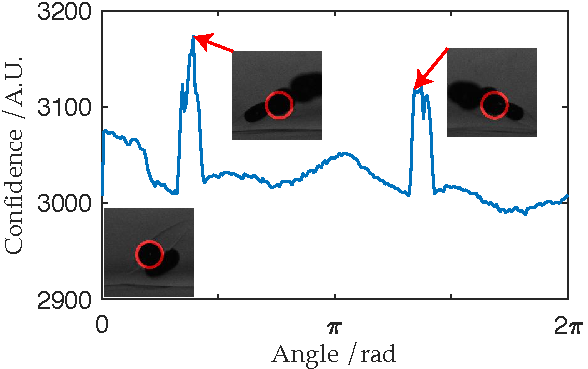
\includegraphics{./figures/results/confidence_bead_tracking}
%   \caption{A plot of the confidence value of a single fiducial bead being tracking \emph{in vivo}.
%   Sharp changes in the confidence value occur when the fiducial bead is occluded.
%   The image at the origin shows the fiducial being tracked well in the first frame.
%   (Images courtesy of Pedro Vallejo)
%   }
%   \label{fig:confidence_bead_tracking}
% \end{figure}

% \subsection{Multiple views tracking}
% The theory backing the proposed algorithm relies on triangulation between two view points.
% In this work the two view points refer to the image at frames \(n\) and \(n+1\).
% However, it is possible to use three separate views (frames \(n\), \(n+1\) and \(n+2\)) to reconstruct a scene, one such approach being quaternion tensors.
% Working with tensors is computationally and mathematically more challenging, but a future iteration of the algorithm presented here may benefit from using three views to provide a more accurate transformation matrix.
% Beyond three views there currently is no mathematical framework at present for four or more views.
% If such tools did exist, it may be possible to make the algorithm described above as non-iterative and essentially a single shot reconstruction from pixels to voxels.

% \subsection{Fiducial free reconstruction}
%
% In computer vision, scenes often do not contain known fiducial marks and so such marks are found between views.
% To find such a correspondences, points with similar local texture are found and matched in between each image. %, many of these such correspondences are found
% This technique is only valid for views with small angles between them, as would be found in \gls{OPT}.
% A similar method could be introduced into the algorithm presented here, as each image should have sufficient texture, particularly when using \gls{tOPT}.
%
% The following chapter will move from improvements in registration using projective matrices and into improvements in resolution using on-camera slit-scanning.

%A future version of this algorithm may be able to use 3 views to produce a more faithful transformation matrix.
%The mathematics for more than three views currently does not exist.


\begin{figure}
  \centering
  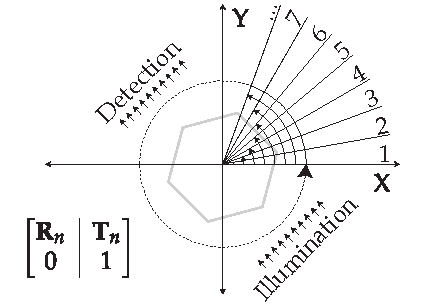
\includegraphics{./figures/flOPT_principle}
  \caption[Principles of the proposed algorithm]{Principles of the proposed algorithm. Each successive frame of \gls{OPT} image data will have an associated \gls{R} and \gls{T} (shown here in augmented form using homogenous coordinates), these matrices can be recovered from comparing the fiducial marker positions in each frame (\(n\)) and its successor (\(n+1\)).}
\end{figure}



\begin{figure}
  \centering
   \hspace*{\fill}
  \begin{subfigure}[t]{0.3\textwidth}
    \begin{tikzpicture}[node distance=0cm]
      \node (img) {
\includegraphics[width=0.8\textwidth]{./figures/results/no_helix/iradon_nofilter}};
       \node[below=of img] {\(X\)};
       \node[left=of img,rotate=90,yshift=0.2cm] {\(Y\)};
    \end{tikzpicture}
    \caption[Unfiltered iRadon]{This is the unfiltered reconstruction of the object using the \gls{Radon transform}}\label{fig:iradon_nofilter}%TODO equation???
  \end{subfigure}\hfill
  \begin{subfigure}[t]{0.3\textwidth}
    \begin{tikzpicture}[node distance=0cm]
      \node (img) {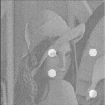
\includegraphics[width=0.8\textwidth]{./figures/results/no_helix/iradon_filter}};
       \node[below=of img] {\(v\)\vphantom{\(X\)}};
       \node[left=of img,rotate=90,yshift=0.2cm] {\(Y\)};
    \end{tikzpicture}
    \caption[Filtered iRadon]{Ram-lak (Fourier ramp) filter applied to \figurename~\ref{fig:iradon_nofilter}.}\label{fig:iradon_filter}
  \end{subfigure}
   \hspace*{\fill}
  \caption[Effects of filtering the result of a inverse Radon transform reconstruction]{
  The result of a tomographic reconstruction (using equally spaced angular steps and no translation between frames) requires Fourier filtering to normalise spatial contrast.}\label{fig:irandons}%TODO simulations with no drift and skew and use equation
\end{figure}


\begin{figure}
  \centering
   \hspace*{\fill}
  \begin{subfigure}[t]{0.3\textwidth}
    \begin{tikzpicture}[node distance=0cm]
      \node (img) {\includegraphics[width=0.8\textwidth]{./figures/results/no_helix/flopt_camerman}};
       \node[below=of img] {\(Z\)};
       \node[left=of img,rotate=90,yshift=0.2cm] {\(Y\)};
    \end{tikzpicture}
    \caption{Filtered reconstruction Cameraman testcard}
  \end{subfigure}\hfill
  \begin{subfigure}[t]{0.3\textwidth}
    \begin{tikzpicture}[node distance=0cm]
      \node (img) {\includegraphics[width=0.8\textwidth]{./figures/results/no_helix/flopt_filter}};
       \node[below=of img] {\(X\)};
       \node[left=of img,rotate=90,yshift=0.2cm] {\(Y\)};
    \end{tikzpicture}
    \caption{Filtered reconstruction of Lena testcard}
  \end{subfigure}
   \hspace*{\fill}
   \caption[Filtered reconstruction of the ground truth reference image using the new proposed algorithm.]{
  Filtered reconstruction of the ground truth reference image from \figurename~\ref{fig:recon_iterative} using the new proposed algorithm.
  }\label{fig:flopt_filter}
\end{figure}


% 
% \begin{figure}
%   \centering
%    \hspace*{\fill}
%   \begin{subfigure}[t]{0.3\textwidth}
%     \begin{tikzpicture}[node distance=0cm]
%       \node (img) {\includegraphics[width=0.8\textwidth]{./figures/results/helix/topdown_bead_paths}};
%        \node[below=of img] {\(X\)};
%        \node[left=of img,rotate=90,yshift=0.2cm] {\(Y\)};
%     \end{tikzpicture}
%     \caption{Top down views (\(X,Y\)) of the source image with the fiducial paths marked.}\label{fig:topdown_bead_paths}
%   \end{subfigure}\hfill
%   \begin{subfigure}[t]{0.3\textwidth}
%     \begin{tikzpicture}[node distance=0cm]
%       \node (img) {\includegraphics[width=0.8\textwidth]{./figures/results/helix/sinugram_stretch}};
%        \node[below=of img] {\(v\)\vphantom{\(X\)}};
%        \node[left=of img,rotate=90,yshift=0.2cm] {\(n\)};
%     \end{tikzpicture}
%     \caption{Sinugram (\(v,n\)) of a sample whose axis of rotation has a systematic drift}\label{fig:flopt_helix_sinugram}
%   \end{subfigure}
%    \hspace*{\fill}
%    \caption{Comparison of the two reconstructions under sample imaging with a systematic drift, in 3D though represented here in 2D.}\label{fig:flopts}
% \end{figure}

% \begin{figure}
%   \centering
%    \hspace*{\fill}
%   \begin{subfigure}[t]{0.3\textwidth}
%     \begin{tikzpicture}[node distance=0cm]
%       \node (img) {\includegraphics[width=0.75\textwidth]{./figures/results/no_helix/rawinput_colour}};
%        \node[below=of img] {\(X\)};
%        \node[left=of img,rotate=90,yshift=0.2cm] {\(Y\)};
%     \end{tikzpicture}
%     \caption{Ground truth image for \gls{OPT} simulations, Lena (\(f(X, Y)\)).}\label{fig:raw_input}
%   \end{subfigure}\hfill
%   \begin{subfigure}[t]{0.3\textwidth}
%     \begin{tikzpicture}[node distance=0cm]
%       \node (img) {\includegraphics[width=0.8\textwidth]{./figures/results/no_helix/sinugram_stretch}};
%        \node[below=of img] {\(v\)\vphantom{\(X\)}};
%        \node[left=of img,rotate=90,yshift=0.2cm] {\(\theta\)};
%     \end{tikzpicture}
%     \caption{Image of Lena (\figurename~\ref{fig:raw_input}) after rotation and projection in 2D, giving the \gls{sinugram} (\(P_{\theta}(v)\)).
%     }\label{fig:sinugram_stretch}
%   \end{subfigure}
%    \hspace*{\fill}
%   \caption{Reference images for \gls{OPT} reconstruction.}\label{fig:rawinputs}
% \end{figure}



\end{document}
